%PROJ3
\chapter{Punkt 2}
%s^{i,j} - ite wyj�cie pod wp�ywem jotego wej�cia

Uzasadni� wyb�r parametr�w optymalizacji.

\begin{figure}[ht]
	\centering
	\begin{tikzpicture}
	\begin{axis}[
	width=5.0in,
	height=3.4in,
	xmin=0,xmax=320,ymin=-0.1,ymax=0.2,
	xlabel={$k$},
	ylabel={$s^{\mathrm{1,1}}$},
	legend pos=south east,
	y tick label style={/pgf/number format/1000 sep=},
	]
	\addplot[const plot,cyan] file {wykresy/przykladowe/zadanie2_sz.txt};
	\end{axis}
	\end{tikzpicture}
	\caption{Odpowied� skokowa wyj�cia 1 przy skoku wej�cia 1}
	\label{odpskokUdmc3}
\end{figure}

\begin{figure}[ht]
	\centering
	\begin{tikzpicture}
	\begin{axis}[
	width=5.0in,
	height=3.4in,
	xmin=0,xmax=320,ymin=-0.1,ymax=0.2,
	xlabel={$k$},
	ylabel={$s^{\mathrm{1,2}}$},
	legend pos=south east,
	y tick label style={/pgf/number format/1000 sep=},
	]
	\addplot[const plot,cyan] file {wykresy/przykladowe/zadanie2_sz.txt};
	\end{axis}
	\end{tikzpicture}
	\caption{Odpowied� skokowa wyj�cia 1 przy skoku wej�cia 2}
	\label{odpskokUdmc3}
\end{figure}

\begin{figure}[ht]
	\centering
	\begin{tikzpicture}
	\begin{axis}[
	width=5.0in,
	height=3.4in,
	xmin=0,xmax=320,ymin=-0.1,ymax=0.2,
	xlabel={$k$},
	ylabel={$s^{\mathrm{2,1}}$},
	legend pos=south east,
	y tick label style={/pgf/number format/1000 sep=},
	]
	\addplot[const plot,cyan] file {wykresy/przykladowe/zadanie2_sz.txt};
	\end{axis}
	\end{tikzpicture}
	\caption{Odpowied� skokowa wyj�cia 2 przy skoku wej�cia 1}
	\label{odpskokUdmc3}
\end{figure}


\begin{figure}[ht]
	\centering
	\begin{tikzpicture}
	\begin{axis}[
	width=5.0in,
	height=3.4in,
	xmin=0,xmax=320,ymin=-0.1,ymax=0.2,
	xlabel={$k$},
	ylabel={$s^{\mathrm{2,2}}$},
	legend pos=south east,
	y tick label style={/pgf/number format/1000 sep=},
	]
	\addplot[const plot,cyan] file {wykresy/przykladowe/zadanie2_sz.txt};
	\end{axis}
	\end{tikzpicture}
	\caption{Odpowied� skokowa wyj�cia 2 przy skoku wej�cia 2}
	\label{odpskokUdmc3}
\end{figure}

\begin{figure}[ht]
	\centering
	\input{./p2_char_stat_1}
	\caption{Charakterystyka statyczna procesu $y_1(u_1,u_2)$}
	\label{Z2c}
\end{figure}

\begin{figure}[ht]
	\centering
	%PROJ3
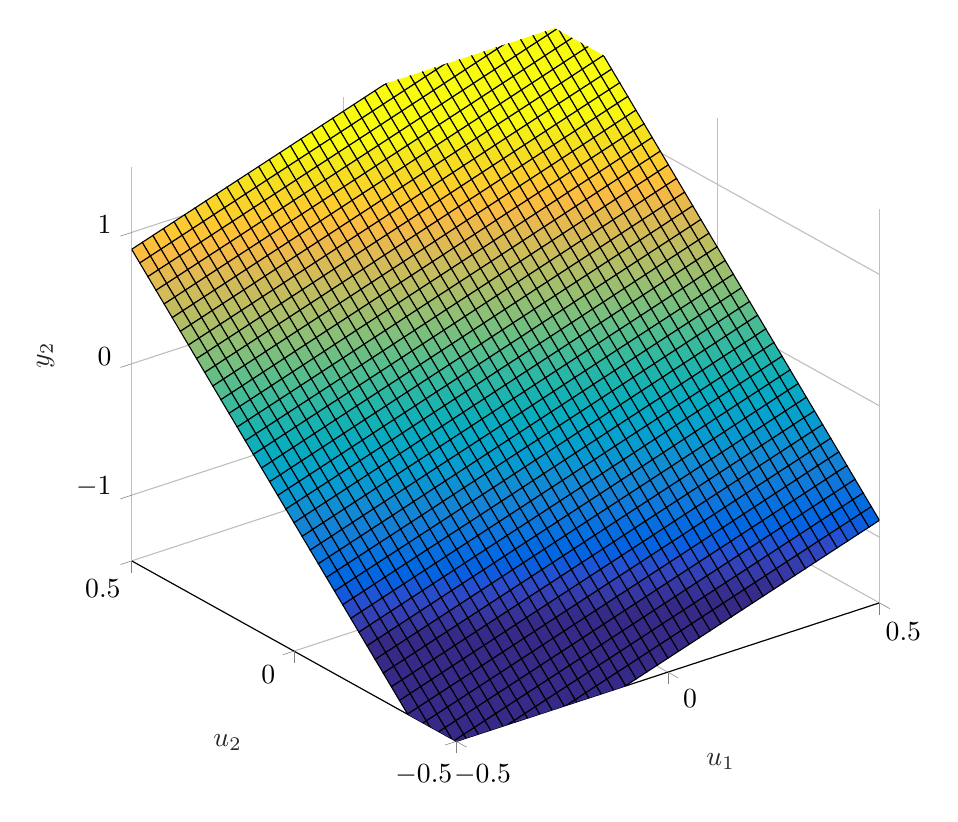
\begin{tikzpicture}

\begin{axis}[%
width=3.739in,
height=3.566in,
at={(0.66in,0.481in)},
scale only axis,
point meta min=-1.19475463603141,
point meta max=1.19475463603141,
xmin=-0.5,
xmax=0.5,
xtick={-0.5,0,0.5},
tick align=outside,
xlabel style={font=\color{white!15!black}},
xlabel={$u_1$},
ymin=-0.5,
ymax=0.5,
ytick={-0.5,0,0.5},
ylabel style={font=\color{white!15!black}},
ylabel={$u_2$},
zmin=-1.5,
zmax=1.5,
zlabel style={font=\color{white!15!black}},
zlabel={$y_2$},
view={-37.5}{30},
axis background/.style={fill=white},
axis x line*=bottom,
axis y line*=left,
axis z line*=left,
xmajorgrids,
ymajorgrids,
zmajorgrids,
colormap={mymap}{[1pt] rgb(0pt)=(0.2081,0.1663,0.5292); rgb(1pt)=(0.211624,0.189781,0.577676); rgb(2pt)=(0.212252,0.213771,0.626971); rgb(3pt)=(0.2081,0.2386,0.677086); rgb(4pt)=(0.195905,0.264457,0.7279); rgb(5pt)=(0.170729,0.291938,0.779248); rgb(6pt)=(0.125271,0.324243,0.830271); rgb(7pt)=(0.0591333,0.359833,0.868333); rgb(8pt)=(0.0116952,0.38751,0.881957); rgb(9pt)=(0.00595714,0.408614,0.882843); rgb(10pt)=(0.0165143,0.4266,0.878633); rgb(11pt)=(0.0328524,0.443043,0.871957); rgb(12pt)=(0.0498143,0.458571,0.864057); rgb(13pt)=(0.0629333,0.47369,0.855438); rgb(14pt)=(0.0722667,0.488667,0.8467); rgb(15pt)=(0.0779429,0.503986,0.838371); rgb(16pt)=(0.0793476,0.520024,0.831181); rgb(17pt)=(0.0749429,0.537543,0.826271); rgb(18pt)=(0.0640571,0.556986,0.823957); rgb(19pt)=(0.0487714,0.577224,0.822829); rgb(20pt)=(0.0343429,0.596581,0.819852); rgb(21pt)=(0.0265,0.6137,0.8135); rgb(22pt)=(0.0238905,0.628662,0.803762); rgb(23pt)=(0.0230905,0.641786,0.791267); rgb(24pt)=(0.0227714,0.653486,0.776757); rgb(25pt)=(0.0266619,0.664195,0.760719); rgb(26pt)=(0.0383714,0.674271,0.743552); rgb(27pt)=(0.0589714,0.683757,0.725386); rgb(28pt)=(0.0843,0.692833,0.706167); rgb(29pt)=(0.113295,0.7015,0.685857); rgb(30pt)=(0.145271,0.709757,0.664629); rgb(31pt)=(0.180133,0.717657,0.642433); rgb(32pt)=(0.217829,0.725043,0.619262); rgb(33pt)=(0.258643,0.731714,0.595429); rgb(34pt)=(0.302171,0.737605,0.571186); rgb(35pt)=(0.348167,0.742433,0.547267); rgb(36pt)=(0.395257,0.7459,0.524443); rgb(37pt)=(0.44201,0.748081,0.503314); rgb(38pt)=(0.487124,0.749062,0.483976); rgb(39pt)=(0.530029,0.749114,0.466114); rgb(40pt)=(0.570857,0.748519,0.44939); rgb(41pt)=(0.609852,0.747314,0.433686); rgb(42pt)=(0.6473,0.7456,0.4188); rgb(43pt)=(0.683419,0.743476,0.404433); rgb(44pt)=(0.71841,0.741133,0.390476); rgb(45pt)=(0.752486,0.7384,0.376814); rgb(46pt)=(0.785843,0.735567,0.363271); rgb(47pt)=(0.818505,0.732733,0.34979); rgb(48pt)=(0.850657,0.7299,0.336029); rgb(49pt)=(0.882433,0.727433,0.3217); rgb(50pt)=(0.913933,0.725786,0.306276); rgb(51pt)=(0.944957,0.726114,0.288643); rgb(52pt)=(0.973895,0.731395,0.266648); rgb(53pt)=(0.993771,0.745457,0.240348); rgb(54pt)=(0.999043,0.765314,0.216414); rgb(55pt)=(0.995533,0.786057,0.196652); rgb(56pt)=(0.988,0.8066,0.179367); rgb(57pt)=(0.978857,0.827143,0.163314); rgb(58pt)=(0.9697,0.848138,0.147452); rgb(59pt)=(0.962586,0.870514,0.1309); rgb(60pt)=(0.958871,0.8949,0.113243); rgb(61pt)=(0.959824,0.921833,0.0948381); rgb(62pt)=(0.9661,0.951443,0.0755333); rgb(63pt)=(0.9763,0.9831,0.0538)},
%colorbar
]

\addplot3[%
surf,
shader=flat corner, draw=black, z buffer=sort, colormap={mymap}{[1pt] rgb(0pt)=(0.2081,0.1663,0.5292); rgb(1pt)=(0.211624,0.189781,0.577676); rgb(2pt)=(0.212252,0.213771,0.626971); rgb(3pt)=(0.2081,0.2386,0.677086); rgb(4pt)=(0.195905,0.264457,0.7279); rgb(5pt)=(0.170729,0.291938,0.779248); rgb(6pt)=(0.125271,0.324243,0.830271); rgb(7pt)=(0.0591333,0.359833,0.868333); rgb(8pt)=(0.0116952,0.38751,0.881957); rgb(9pt)=(0.00595714,0.408614,0.882843); rgb(10pt)=(0.0165143,0.4266,0.878633); rgb(11pt)=(0.0328524,0.443043,0.871957); rgb(12pt)=(0.0498143,0.458571,0.864057); rgb(13pt)=(0.0629333,0.47369,0.855438); rgb(14pt)=(0.0722667,0.488667,0.8467); rgb(15pt)=(0.0779429,0.503986,0.838371); rgb(16pt)=(0.0793476,0.520024,0.831181); rgb(17pt)=(0.0749429,0.537543,0.826271); rgb(18pt)=(0.0640571,0.556986,0.823957); rgb(19pt)=(0.0487714,0.577224,0.822829); rgb(20pt)=(0.0343429,0.596581,0.819852); rgb(21pt)=(0.0265,0.6137,0.8135); rgb(22pt)=(0.0238905,0.628662,0.803762); rgb(23pt)=(0.0230905,0.641786,0.791267); rgb(24pt)=(0.0227714,0.653486,0.776757); rgb(25pt)=(0.0266619,0.664195,0.760719); rgb(26pt)=(0.0383714,0.674271,0.743552); rgb(27pt)=(0.0589714,0.683757,0.725386); rgb(28pt)=(0.0843,0.692833,0.706167); rgb(29pt)=(0.113295,0.7015,0.685857); rgb(30pt)=(0.145271,0.709757,0.664629); rgb(31pt)=(0.180133,0.717657,0.642433); rgb(32pt)=(0.217829,0.725043,0.619262); rgb(33pt)=(0.258643,0.731714,0.595429); rgb(34pt)=(0.302171,0.737605,0.571186); rgb(35pt)=(0.348167,0.742433,0.547267); rgb(36pt)=(0.395257,0.7459,0.524443); rgb(37pt)=(0.44201,0.748081,0.503314); rgb(38pt)=(0.487124,0.749062,0.483976); rgb(39pt)=(0.530029,0.749114,0.466114); rgb(40pt)=(0.570857,0.748519,0.44939); rgb(41pt)=(0.609852,0.747314,0.433686); rgb(42pt)=(0.6473,0.7456,0.4188); rgb(43pt)=(0.683419,0.743476,0.404433); rgb(44pt)=(0.71841,0.741133,0.390476); rgb(45pt)=(0.752486,0.7384,0.376814); rgb(46pt)=(0.785843,0.735567,0.363271); rgb(47pt)=(0.818505,0.732733,0.34979); rgb(48pt)=(0.850657,0.7299,0.336029); rgb(49pt)=(0.882433,0.727433,0.3217); rgb(50pt)=(0.913933,0.725786,0.306276); rgb(51pt)=(0.944957,0.726114,0.288643); rgb(52pt)=(0.973895,0.731395,0.266648); rgb(53pt)=(0.993771,0.745457,0.240348); rgb(54pt)=(0.999043,0.765314,0.216414); rgb(55pt)=(0.995533,0.786057,0.196652); rgb(56pt)=(0.988,0.8066,0.179367); rgb(57pt)=(0.978857,0.827143,0.163314); rgb(58pt)=(0.9697,0.848138,0.147452); rgb(59pt)=(0.962586,0.870514,0.1309); rgb(60pt)=(0.958871,0.8949,0.113243); rgb(61pt)=(0.959824,0.921833,0.0948381); rgb(62pt)=(0.9661,0.951443,0.0755333); rgb(63pt)=(0.9763,0.9831,0.0538)}, mesh/rows=41]
table[row sep=crcr, point meta=\thisrow{c}] {%
%
%x - w prawo poziomo (G1?)
%y - w lewo poziomo (G2?)
%z - w g�r� (T3?)
%c - kopia z
x	y	z	c\\
-0.500000	-0.500000	-1.917004	-1.917004\\ 
-0.500000	-0.475000	-1.847289	-1.847289\\ 
-0.500000	-0.450000	-1.777574	-1.777574\\ 
-0.500000	-0.425000	-1.707858	-1.707858\\ 
-0.500000	-0.400000	-1.638143	-1.638143\\ 
-0.500000	-0.375000	-1.568428	-1.568428\\ 
-0.500000	-0.350000	-1.498713	-1.498713\\ 
-0.500000	-0.325000	-1.428998	-1.428998\\ 
-0.500000	-0.300000	-1.359283	-1.359283\\ 
-0.500000	-0.275000	-1.289568	-1.289568\\ 
-0.500000	-0.250000	-1.219853	-1.219853\\ 
-0.500000	-0.225000	-1.150138	-1.150138\\ 
-0.500000	-0.200000	-1.080423	-1.080423\\ 
-0.500000	-0.175000	-1.010708	-1.010708\\ 
-0.500000	-0.150000	-0.940993	-0.940993\\ 
-0.500000	-0.125000	-0.871278	-0.871278\\ 
-0.500000	-0.100000	-0.801562	-0.801562\\ 
-0.500000	-0.075000	-0.731847	-0.731847\\ 
-0.500000	-0.050000	-0.662132	-0.662132\\ 
-0.500000	-0.025000	-0.592417	-0.592417\\ 
-0.500000	0.000000	-0.522702	-0.522702\\ 
-0.500000	0.025000	-0.452987	-0.452987\\ 
-0.500000	0.050000	-0.383272	-0.383272\\ 
-0.500000	0.075000	-0.313557	-0.313557\\ 
-0.500000	0.100000	-0.243842	-0.243842\\ 
-0.500000	0.125000	-0.174127	-0.174127\\ 
-0.500000	0.150000	-0.104412	-0.104412\\ 
-0.500000	0.175000	-0.034697	-0.034697\\ 
-0.500000	0.200000	0.035018	0.035018\\ 
-0.500000	0.225000	0.104733	0.104733\\ 
-0.500000	0.250000	0.174449	0.174449\\ 
-0.500000	0.275000	0.244164	0.244164\\ 
-0.500000	0.300000	0.313879	0.313879\\ 
-0.500000	0.325000	0.383594	0.383594\\ 
-0.500000	0.350000	0.453309	0.453309\\ 
-0.500000	0.375000	0.523024	0.523024\\ 
-0.500000	0.400000	0.592739	0.592739\\ 
-0.500000	0.425000	0.662454	0.662454\\ 
-0.500000	0.450000	0.732169	0.732169\\ 
-0.500000	0.475000	0.801884	0.801884\\ 
-0.500000	0.500000	0.871599	0.871599\\ 
-0.475000	-0.500000	-1.890869	-1.890869\\ 
-0.475000	-0.475000	-1.821153	-1.821153\\ 
-0.475000	-0.450000	-1.751438	-1.751438\\ 
-0.475000	-0.425000	-1.681723	-1.681723\\ 
-0.475000	-0.400000	-1.612008	-1.612008\\ 
-0.475000	-0.375000	-1.542293	-1.542293\\ 
-0.475000	-0.350000	-1.472578	-1.472578\\ 
-0.475000	-0.325000	-1.402863	-1.402863\\ 
-0.475000	-0.300000	-1.333148	-1.333148\\ 
-0.475000	-0.275000	-1.263433	-1.263433\\ 
-0.475000	-0.250000	-1.193718	-1.193718\\ 
-0.475000	-0.225000	-1.124003	-1.124003\\ 
-0.475000	-0.200000	-1.054288	-1.054288\\ 
-0.475000	-0.175000	-0.984573	-0.984573\\ 
-0.475000	-0.150000	-0.914858	-0.914858\\ 
-0.475000	-0.125000	-0.845142	-0.845142\\ 
-0.475000	-0.100000	-0.775427	-0.775427\\ 
-0.475000	-0.075000	-0.705712	-0.705712\\ 
-0.475000	-0.050000	-0.635997	-0.635997\\ 
-0.475000	-0.025000	-0.566282	-0.566282\\ 
-0.475000	0.000000	-0.496567	-0.496567\\ 
-0.475000	0.025000	-0.426852	-0.426852\\ 
-0.475000	0.050000	-0.357137	-0.357137\\ 
-0.475000	0.075000	-0.287422	-0.287422\\ 
-0.475000	0.100000	-0.217707	-0.217707\\ 
-0.475000	0.125000	-0.147992	-0.147992\\ 
-0.475000	0.150000	-0.078277	-0.078277\\ 
-0.475000	0.175000	-0.008562	-0.008562\\ 
-0.475000	0.200000	0.061153	0.061153\\ 
-0.475000	0.225000	0.130869	0.130869\\ 
-0.475000	0.250000	0.200584	0.200584\\ 
-0.475000	0.275000	0.270299	0.270299\\ 
-0.475000	0.300000	0.340014	0.340014\\ 
-0.475000	0.325000	0.409729	0.409729\\ 
-0.475000	0.350000	0.479444	0.479444\\ 
-0.475000	0.375000	0.549159	0.549159\\ 
-0.475000	0.400000	0.618874	0.618874\\ 
-0.475000	0.425000	0.688589	0.688589\\ 
-0.475000	0.450000	0.758304	0.758304\\ 
-0.475000	0.475000	0.828019	0.828019\\ 
-0.475000	0.500000	0.897734	0.897734\\ 
-0.450000	-0.500000	-1.864733	-1.864733\\ 
-0.450000	-0.475000	-1.795018	-1.795018\\ 
-0.450000	-0.450000	-1.725303	-1.725303\\ 
-0.450000	-0.425000	-1.655588	-1.655588\\ 
-0.450000	-0.400000	-1.585873	-1.585873\\ 
-0.450000	-0.375000	-1.516158	-1.516158\\ 
-0.450000	-0.350000	-1.446443	-1.446443\\ 
-0.450000	-0.325000	-1.376728	-1.376728\\ 
-0.450000	-0.300000	-1.307013	-1.307013\\ 
-0.450000	-0.275000	-1.237298	-1.237298\\ 
-0.450000	-0.250000	-1.167583	-1.167583\\ 
-0.450000	-0.225000	-1.097868	-1.097868\\ 
-0.450000	-0.200000	-1.028153	-1.028153\\ 
-0.450000	-0.175000	-0.958437	-0.958437\\ 
-0.450000	-0.150000	-0.888722	-0.888722\\ 
-0.450000	-0.125000	-0.819007	-0.819007\\ 
-0.450000	-0.100000	-0.749292	-0.749292\\ 
-0.450000	-0.075000	-0.679577	-0.679577\\ 
-0.450000	-0.050000	-0.609862	-0.609862\\ 
-0.450000	-0.025000	-0.540147	-0.540147\\ 
-0.450000	0.000000	-0.470432	-0.470432\\ 
-0.450000	0.025000	-0.400717	-0.400717\\ 
-0.450000	0.050000	-0.331002	-0.331002\\ 
-0.450000	0.075000	-0.261287	-0.261287\\ 
-0.450000	0.100000	-0.191572	-0.191572\\ 
-0.450000	0.125000	-0.121857	-0.121857\\ 
-0.450000	0.150000	-0.052142	-0.052142\\ 
-0.450000	0.175000	0.017574	0.017574\\ 
-0.450000	0.200000	0.087289	0.087289\\ 
-0.450000	0.225000	0.157004	0.157004\\ 
-0.450000	0.250000	0.226719	0.226719\\ 
-0.450000	0.275000	0.296434	0.296434\\ 
-0.450000	0.300000	0.366149	0.366149\\ 
-0.450000	0.325000	0.435864	0.435864\\ 
-0.450000	0.350000	0.505579	0.505579\\ 
-0.450000	0.375000	0.575294	0.575294\\ 
-0.450000	0.400000	0.645009	0.645009\\ 
-0.450000	0.425000	0.714724	0.714724\\ 
-0.450000	0.450000	0.784439	0.784439\\ 
-0.450000	0.475000	0.854154	0.854154\\ 
-0.450000	0.500000	0.923869	0.923869\\ 
-0.425000	-0.500000	-1.838598	-1.838598\\ 
-0.425000	-0.475000	-1.768883	-1.768883\\ 
-0.425000	-0.450000	-1.699168	-1.699168\\ 
-0.425000	-0.425000	-1.629453	-1.629453\\ 
-0.425000	-0.400000	-1.559738	-1.559738\\ 
-0.425000	-0.375000	-1.490023	-1.490023\\ 
-0.425000	-0.350000	-1.420308	-1.420308\\ 
-0.425000	-0.325000	-1.350593	-1.350593\\ 
-0.425000	-0.300000	-1.280878	-1.280878\\ 
-0.425000	-0.275000	-1.211163	-1.211163\\ 
-0.425000	-0.250000	-1.141448	-1.141448\\ 
-0.425000	-0.225000	-1.071733	-1.071733\\ 
-0.425000	-0.200000	-1.002017	-1.002017\\ 
-0.425000	-0.175000	-0.932302	-0.932302\\ 
-0.425000	-0.150000	-0.862587	-0.862587\\ 
-0.425000	-0.125000	-0.792872	-0.792872\\ 
-0.425000	-0.100000	-0.723157	-0.723157\\ 
-0.425000	-0.075000	-0.653442	-0.653442\\ 
-0.425000	-0.050000	-0.583727	-0.583727\\ 
-0.425000	-0.025000	-0.514012	-0.514012\\ 
-0.425000	0.000000	-0.444297	-0.444297\\ 
-0.425000	0.025000	-0.374582	-0.374582\\ 
-0.425000	0.050000	-0.304867	-0.304867\\ 
-0.425000	0.075000	-0.235152	-0.235152\\ 
-0.425000	0.100000	-0.165437	-0.165437\\ 
-0.425000	0.125000	-0.095722	-0.095722\\ 
-0.425000	0.150000	-0.026006	-0.026006\\ 
-0.425000	0.175000	0.043709	0.043709\\ 
-0.425000	0.200000	0.113424	0.113424\\ 
-0.425000	0.225000	0.183139	0.183139\\ 
-0.425000	0.250000	0.252854	0.252854\\ 
-0.425000	0.275000	0.322569	0.322569\\ 
-0.425000	0.300000	0.392284	0.392284\\ 
-0.425000	0.325000	0.461999	0.461999\\ 
-0.425000	0.350000	0.531714	0.531714\\ 
-0.425000	0.375000	0.601429	0.601429\\ 
-0.425000	0.400000	0.671144	0.671144\\ 
-0.425000	0.425000	0.740859	0.740859\\ 
-0.425000	0.450000	0.810574	0.810574\\ 
-0.425000	0.475000	0.880290	0.880290\\ 
-0.425000	0.500000	0.950005	0.950005\\ 
-0.400000	-0.500000	-1.812463	-1.812463\\ 
-0.400000	-0.475000	-1.742748	-1.742748\\ 
-0.400000	-0.450000	-1.673033	-1.673033\\ 
-0.400000	-0.425000	-1.603318	-1.603318\\ 
-0.400000	-0.400000	-1.533603	-1.533603\\ 
-0.400000	-0.375000	-1.463888	-1.463888\\ 
-0.400000	-0.350000	-1.394173	-1.394173\\ 
-0.400000	-0.325000	-1.324458	-1.324458\\ 
-0.400000	-0.300000	-1.254743	-1.254743\\ 
-0.400000	-0.275000	-1.185028	-1.185028\\ 
-0.400000	-0.250000	-1.115312	-1.115312\\ 
-0.400000	-0.225000	-1.045597	-1.045597\\ 
-0.400000	-0.200000	-0.975882	-0.975882\\ 
-0.400000	-0.175000	-0.906167	-0.906167\\ 
-0.400000	-0.150000	-0.836452	-0.836452\\ 
-0.400000	-0.125000	-0.766737	-0.766737\\ 
-0.400000	-0.100000	-0.697022	-0.697022\\ 
-0.400000	-0.075000	-0.627307	-0.627307\\ 
-0.400000	-0.050000	-0.557592	-0.557592\\ 
-0.400000	-0.025000	-0.487877	-0.487877\\ 
-0.400000	0.000000	-0.418162	-0.418162\\ 
-0.400000	0.025000	-0.348447	-0.348447\\ 
-0.400000	0.050000	-0.278732	-0.278732\\ 
-0.400000	0.075000	-0.209017	-0.209017\\ 
-0.400000	0.100000	-0.139301	-0.139301\\ 
-0.400000	0.125000	-0.069586	-0.069586\\ 
-0.400000	0.150000	0.000129	0.000129\\ 
-0.400000	0.175000	0.069844	0.069844\\ 
-0.400000	0.200000	0.139559	0.139559\\ 
-0.400000	0.225000	0.209274	0.209274\\ 
-0.400000	0.250000	0.278989	0.278989\\ 
-0.400000	0.275000	0.348704	0.348704\\ 
-0.400000	0.300000	0.418419	0.418419\\ 
-0.400000	0.325000	0.488134	0.488134\\ 
-0.400000	0.350000	0.557849	0.557849\\ 
-0.400000	0.375000	0.627564	0.627564\\ 
-0.400000	0.400000	0.697279	0.697279\\ 
-0.400000	0.425000	0.766994	0.766994\\ 
-0.400000	0.450000	0.836710	0.836710\\ 
-0.400000	0.475000	0.906425	0.906425\\ 
-0.400000	0.500000	0.976140	0.976140\\ 
-0.375000	-0.500000	-1.786328	-1.786328\\ 
-0.375000	-0.475000	-1.716613	-1.716613\\ 
-0.375000	-0.450000	-1.646898	-1.646898\\ 
-0.375000	-0.425000	-1.577183	-1.577183\\ 
-0.375000	-0.400000	-1.507468	-1.507468\\ 
-0.375000	-0.375000	-1.437753	-1.437753\\ 
-0.375000	-0.350000	-1.368038	-1.368038\\ 
-0.375000	-0.325000	-1.298323	-1.298323\\ 
-0.375000	-0.300000	-1.228608	-1.228608\\ 
-0.375000	-0.275000	-1.158892	-1.158892\\ 
-0.375000	-0.250000	-1.089177	-1.089177\\ 
-0.375000	-0.225000	-1.019462	-1.019462\\ 
-0.375000	-0.200000	-0.949747	-0.949747\\ 
-0.375000	-0.175000	-0.880032	-0.880032\\ 
-0.375000	-0.150000	-0.810317	-0.810317\\ 
-0.375000	-0.125000	-0.740602	-0.740602\\ 
-0.375000	-0.100000	-0.670887	-0.670887\\ 
-0.375000	-0.075000	-0.601172	-0.601172\\ 
-0.375000	-0.050000	-0.531457	-0.531457\\ 
-0.375000	-0.025000	-0.461742	-0.461742\\ 
-0.375000	0.000000	-0.392027	-0.392027\\ 
-0.375000	0.025000	-0.322312	-0.322312\\ 
-0.375000	0.050000	-0.252597	-0.252597\\ 
-0.375000	0.075000	-0.182881	-0.182881\\ 
-0.375000	0.100000	-0.113166	-0.113166\\ 
-0.375000	0.125000	-0.043451	-0.043451\\ 
-0.375000	0.150000	0.026264	0.026264\\ 
-0.375000	0.175000	0.095979	0.095979\\ 
-0.375000	0.200000	0.165694	0.165694\\ 
-0.375000	0.225000	0.235409	0.235409\\ 
-0.375000	0.250000	0.305124	0.305124\\ 
-0.375000	0.275000	0.374839	0.374839\\ 
-0.375000	0.300000	0.444554	0.444554\\ 
-0.375000	0.325000	0.514269	0.514269\\ 
-0.375000	0.350000	0.583984	0.583984\\ 
-0.375000	0.375000	0.653699	0.653699\\ 
-0.375000	0.400000	0.723415	0.723415\\ 
-0.375000	0.425000	0.793130	0.793130\\ 
-0.375000	0.450000	0.862845	0.862845\\ 
-0.375000	0.475000	0.932560	0.932560\\ 
-0.375000	0.500000	1.002275	1.002275\\ 
-0.350000	-0.500000	-1.760193	-1.760193\\ 
-0.350000	-0.475000	-1.690478	-1.690478\\ 
-0.350000	-0.450000	-1.620763	-1.620763\\ 
-0.350000	-0.425000	-1.551048	-1.551048\\ 
-0.350000	-0.400000	-1.481333	-1.481333\\ 
-0.350000	-0.375000	-1.411618	-1.411618\\ 
-0.350000	-0.350000	-1.341903	-1.341903\\ 
-0.350000	-0.325000	-1.272187	-1.272187\\ 
-0.350000	-0.300000	-1.202472	-1.202472\\ 
-0.350000	-0.275000	-1.132757	-1.132757\\ 
-0.350000	-0.250000	-1.063042	-1.063042\\ 
-0.350000	-0.225000	-0.993327	-0.993327\\ 
-0.350000	-0.200000	-0.923612	-0.923612\\ 
-0.350000	-0.175000	-0.853897	-0.853897\\ 
-0.350000	-0.150000	-0.784182	-0.784182\\ 
-0.350000	-0.125000	-0.714467	-0.714467\\ 
-0.350000	-0.100000	-0.644752	-0.644752\\ 
-0.350000	-0.075000	-0.575037	-0.575037\\ 
-0.350000	-0.050000	-0.505322	-0.505322\\ 
-0.350000	-0.025000	-0.435607	-0.435607\\ 
-0.350000	0.000000	-0.365892	-0.365892\\ 
-0.350000	0.025000	-0.296176	-0.296176\\ 
-0.350000	0.050000	-0.226461	-0.226461\\ 
-0.350000	0.075000	-0.156746	-0.156746\\ 
-0.350000	0.100000	-0.087031	-0.087031\\ 
-0.350000	0.125000	-0.017316	-0.017316\\ 
-0.350000	0.150000	0.052399	0.052399\\ 
-0.350000	0.175000	0.122114	0.122114\\ 
-0.350000	0.200000	0.191829	0.191829\\ 
-0.350000	0.225000	0.261544	0.261544\\ 
-0.350000	0.250000	0.331259	0.331259\\ 
-0.350000	0.275000	0.400974	0.400974\\ 
-0.350000	0.300000	0.470689	0.470689\\ 
-0.350000	0.325000	0.540404	0.540404\\ 
-0.350000	0.350000	0.610119	0.610119\\ 
-0.350000	0.375000	0.679835	0.679835\\ 
-0.350000	0.400000	0.749550	0.749550\\ 
-0.350000	0.425000	0.819265	0.819265\\ 
-0.350000	0.450000	0.888980	0.888980\\ 
-0.350000	0.475000	0.958695	0.958695\\ 
-0.350000	0.500000	1.028410	1.028410\\ 
-0.325000	-0.500000	-1.734058	-1.734058\\ 
-0.325000	-0.475000	-1.664343	-1.664343\\ 
-0.325000	-0.450000	-1.594628	-1.594628\\ 
-0.325000	-0.425000	-1.524913	-1.524913\\ 
-0.325000	-0.400000	-1.455198	-1.455198\\ 
-0.325000	-0.375000	-1.385483	-1.385483\\ 
-0.325000	-0.350000	-1.315767	-1.315767\\ 
-0.325000	-0.325000	-1.246052	-1.246052\\ 
-0.325000	-0.300000	-1.176337	-1.176337\\ 
-0.325000	-0.275000	-1.106622	-1.106622\\ 
-0.325000	-0.250000	-1.036907	-1.036907\\ 
-0.325000	-0.225000	-0.967192	-0.967192\\ 
-0.325000	-0.200000	-0.897477	-0.897477\\ 
-0.325000	-0.175000	-0.827762	-0.827762\\ 
-0.325000	-0.150000	-0.758047	-0.758047\\ 
-0.325000	-0.125000	-0.688332	-0.688332\\ 
-0.325000	-0.100000	-0.618617	-0.618617\\ 
-0.325000	-0.075000	-0.548902	-0.548902\\ 
-0.325000	-0.050000	-0.479187	-0.479187\\ 
-0.325000	-0.025000	-0.409472	-0.409472\\ 
-0.325000	0.000000	-0.339756	-0.339756\\ 
-0.325000	0.025000	-0.270041	-0.270041\\ 
-0.325000	0.050000	-0.200326	-0.200326\\ 
-0.325000	0.075000	-0.130611	-0.130611\\ 
-0.325000	0.100000	-0.060896	-0.060896\\ 
-0.325000	0.125000	0.008819	0.008819\\ 
-0.325000	0.150000	0.078534	0.078534\\ 
-0.325000	0.175000	0.148249	0.148249\\ 
-0.325000	0.200000	0.217964	0.217964\\ 
-0.325000	0.225000	0.287679	0.287679\\ 
-0.325000	0.250000	0.357394	0.357394\\ 
-0.325000	0.275000	0.427109	0.427109\\ 
-0.325000	0.300000	0.496824	0.496824\\ 
-0.325000	0.325000	0.566540	0.566540\\ 
-0.325000	0.350000	0.636255	0.636255\\ 
-0.325000	0.375000	0.705970	0.705970\\ 
-0.325000	0.400000	0.775685	0.775685\\ 
-0.325000	0.425000	0.845400	0.845400\\ 
-0.325000	0.450000	0.915115	0.915115\\ 
-0.325000	0.475000	0.984830	0.984830\\ 
-0.325000	0.500000	1.054545	1.054545\\ 
-0.300000	-0.500000	-1.707923	-1.707923\\ 
-0.300000	-0.475000	-1.638208	-1.638208\\ 
-0.300000	-0.450000	-1.568493	-1.568493\\ 
-0.300000	-0.425000	-1.498778	-1.498778\\ 
-0.300000	-0.400000	-1.429062	-1.429062\\ 
-0.300000	-0.375000	-1.359347	-1.359347\\ 
-0.300000	-0.350000	-1.289632	-1.289632\\ 
-0.300000	-0.325000	-1.219917	-1.219917\\ 
-0.300000	-0.300000	-1.150202	-1.150202\\ 
-0.300000	-0.275000	-1.080487	-1.080487\\ 
-0.300000	-0.250000	-1.010772	-1.010772\\ 
-0.300000	-0.225000	-0.941057	-0.941057\\ 
-0.300000	-0.200000	-0.871342	-0.871342\\ 
-0.300000	-0.175000	-0.801627	-0.801627\\ 
-0.300000	-0.150000	-0.731912	-0.731912\\ 
-0.300000	-0.125000	-0.662197	-0.662197\\ 
-0.300000	-0.100000	-0.592482	-0.592482\\ 
-0.300000	-0.075000	-0.522767	-0.522767\\ 
-0.300000	-0.050000	-0.453051	-0.453051\\ 
-0.300000	-0.025000	-0.383336	-0.383336\\ 
-0.300000	0.000000	-0.313621	-0.313621\\ 
-0.300000	0.025000	-0.243906	-0.243906\\ 
-0.300000	0.050000	-0.174191	-0.174191\\ 
-0.300000	0.075000	-0.104476	-0.104476\\ 
-0.300000	0.100000	-0.034761	-0.034761\\ 
-0.300000	0.125000	0.034954	0.034954\\ 
-0.300000	0.150000	0.104669	0.104669\\ 
-0.300000	0.175000	0.174384	0.174384\\ 
-0.300000	0.200000	0.244099	0.244099\\ 
-0.300000	0.225000	0.313814	0.313814\\ 
-0.300000	0.250000	0.383529	0.383529\\ 
-0.300000	0.275000	0.453244	0.453244\\ 
-0.300000	0.300000	0.522960	0.522960\\ 
-0.300000	0.325000	0.592675	0.592675\\ 
-0.300000	0.350000	0.662390	0.662390\\ 
-0.300000	0.375000	0.732105	0.732105\\ 
-0.300000	0.400000	0.801820	0.801820\\ 
-0.300000	0.425000	0.871535	0.871535\\ 
-0.300000	0.450000	0.941250	0.941250\\ 
-0.300000	0.475000	1.010965	1.010965\\ 
-0.300000	0.500000	1.080680	1.080680\\ 
-0.275000	-0.500000	-1.681788	-1.681788\\ 
-0.275000	-0.475000	-1.612073	-1.612073\\ 
-0.275000	-0.450000	-1.542358	-1.542358\\ 
-0.275000	-0.425000	-1.472642	-1.472642\\ 
-0.275000	-0.400000	-1.402927	-1.402927\\ 
-0.275000	-0.375000	-1.333212	-1.333212\\ 
-0.275000	-0.350000	-1.263497	-1.263497\\ 
-0.275000	-0.325000	-1.193782	-1.193782\\ 
-0.275000	-0.300000	-1.124067	-1.124067\\ 
-0.275000	-0.275000	-1.054352	-1.054352\\ 
-0.275000	-0.250000	-0.984637	-0.984637\\ 
-0.275000	-0.225000	-0.914922	-0.914922\\ 
-0.275000	-0.200000	-0.845207	-0.845207\\ 
-0.275000	-0.175000	-0.775492	-0.775492\\ 
-0.275000	-0.150000	-0.705777	-0.705777\\ 
-0.275000	-0.125000	-0.636062	-0.636062\\ 
-0.275000	-0.100000	-0.566347	-0.566347\\ 
-0.275000	-0.075000	-0.496631	-0.496631\\ 
-0.275000	-0.050000	-0.426916	-0.426916\\ 
-0.275000	-0.025000	-0.357201	-0.357201\\ 
-0.275000	0.000000	-0.287486	-0.287486\\ 
-0.275000	0.025000	-0.217771	-0.217771\\ 
-0.275000	0.050000	-0.148056	-0.148056\\ 
-0.275000	0.075000	-0.078341	-0.078341\\ 
-0.275000	0.100000	-0.008626	-0.008626\\ 
-0.275000	0.125000	0.061089	0.061089\\ 
-0.275000	0.150000	0.130804	0.130804\\ 
-0.275000	0.175000	0.200519	0.200519\\ 
-0.275000	0.200000	0.270234	0.270234\\ 
-0.275000	0.225000	0.339949	0.339949\\ 
-0.275000	0.250000	0.409665	0.409665\\ 
-0.275000	0.275000	0.479380	0.479380\\ 
-0.275000	0.300000	0.549095	0.549095\\ 
-0.275000	0.325000	0.618810	0.618810\\ 
-0.275000	0.350000	0.688525	0.688525\\ 
-0.275000	0.375000	0.758240	0.758240\\ 
-0.275000	0.400000	0.827955	0.827955\\ 
-0.275000	0.425000	0.897670	0.897670\\ 
-0.275000	0.450000	0.967385	0.967385\\ 
-0.275000	0.475000	1.037100	1.037100\\ 
-0.275000	0.500000	1.106815	1.106815\\ 
-0.250000	-0.500000	-1.655653	-1.655653\\ 
-0.250000	-0.475000	-1.585937	-1.585937\\ 
-0.250000	-0.450000	-1.516222	-1.516222\\ 
-0.250000	-0.425000	-1.446507	-1.446507\\ 
-0.250000	-0.400000	-1.376792	-1.376792\\ 
-0.250000	-0.375000	-1.307077	-1.307077\\ 
-0.250000	-0.350000	-1.237362	-1.237362\\ 
-0.250000	-0.325000	-1.167647	-1.167647\\ 
-0.250000	-0.300000	-1.097932	-1.097932\\ 
-0.250000	-0.275000	-1.028217	-1.028217\\ 
-0.250000	-0.250000	-0.958502	-0.958502\\ 
-0.250000	-0.225000	-0.888787	-0.888787\\ 
-0.250000	-0.200000	-0.819072	-0.819072\\ 
-0.250000	-0.175000	-0.749357	-0.749357\\ 
-0.250000	-0.150000	-0.679642	-0.679642\\ 
-0.250000	-0.125000	-0.609926	-0.609926\\ 
-0.250000	-0.100000	-0.540211	-0.540211\\ 
-0.250000	-0.075000	-0.470496	-0.470496\\ 
-0.250000	-0.050000	-0.400781	-0.400781\\ 
-0.250000	-0.025000	-0.331066	-0.331066\\ 
-0.250000	0.000000	-0.261351	-0.261351\\ 
-0.250000	0.025000	-0.191636	-0.191636\\ 
-0.250000	0.050000	-0.121921	-0.121921\\ 
-0.250000	0.075000	-0.052206	-0.052206\\ 
-0.250000	0.100000	0.017509	0.017509\\ 
-0.250000	0.125000	0.087224	0.087224\\ 
-0.250000	0.150000	0.156939	0.156939\\ 
-0.250000	0.175000	0.226654	0.226654\\ 
-0.250000	0.200000	0.296369	0.296369\\ 
-0.250000	0.225000	0.366085	0.366085\\ 
-0.250000	0.250000	0.435800	0.435800\\ 
-0.250000	0.275000	0.505515	0.505515\\ 
-0.250000	0.300000	0.575230	0.575230\\ 
-0.250000	0.325000	0.644945	0.644945\\ 
-0.250000	0.350000	0.714660	0.714660\\ 
-0.250000	0.375000	0.784375	0.784375\\ 
-0.250000	0.400000	0.854090	0.854090\\ 
-0.250000	0.425000	0.923805	0.923805\\ 
-0.250000	0.450000	0.993520	0.993520\\ 
-0.250000	0.475000	1.063235	1.063235\\ 
-0.250000	0.500000	1.132950	1.132950\\ 
-0.225000	-0.500000	-1.629517	-1.629517\\ 
-0.225000	-0.475000	-1.559802	-1.559802\\ 
-0.225000	-0.450000	-1.490087	-1.490087\\ 
-0.225000	-0.425000	-1.420372	-1.420372\\ 
-0.225000	-0.400000	-1.350657	-1.350657\\ 
-0.225000	-0.375000	-1.280942	-1.280942\\ 
-0.225000	-0.350000	-1.211227	-1.211227\\ 
-0.225000	-0.325000	-1.141512	-1.141512\\ 
-0.225000	-0.300000	-1.071797	-1.071797\\ 
-0.225000	-0.275000	-1.002082	-1.002082\\ 
-0.225000	-0.250000	-0.932367	-0.932367\\ 
-0.225000	-0.225000	-0.862652	-0.862652\\ 
-0.225000	-0.200000	-0.792937	-0.792937\\ 
-0.225000	-0.175000	-0.723222	-0.723222\\ 
-0.225000	-0.150000	-0.653506	-0.653506\\ 
-0.225000	-0.125000	-0.583791	-0.583791\\ 
-0.225000	-0.100000	-0.514076	-0.514076\\ 
-0.225000	-0.075000	-0.444361	-0.444361\\ 
-0.225000	-0.050000	-0.374646	-0.374646\\ 
-0.225000	-0.025000	-0.304931	-0.304931\\ 
-0.225000	0.000000	-0.235216	-0.235216\\ 
-0.225000	0.025000	-0.165501	-0.165501\\ 
-0.225000	0.050000	-0.095786	-0.095786\\ 
-0.225000	0.075000	-0.026071	-0.026071\\ 
-0.225000	0.100000	0.043644	0.043644\\ 
-0.225000	0.125000	0.113359	0.113359\\ 
-0.225000	0.150000	0.183074	0.183074\\ 
-0.225000	0.175000	0.252790	0.252790\\ 
-0.225000	0.200000	0.322505	0.322505\\ 
-0.225000	0.225000	0.392220	0.392220\\ 
-0.225000	0.250000	0.461935	0.461935\\ 
-0.225000	0.275000	0.531650	0.531650\\ 
-0.225000	0.300000	0.601365	0.601365\\ 
-0.225000	0.325000	0.671080	0.671080\\ 
-0.225000	0.350000	0.740795	0.740795\\ 
-0.225000	0.375000	0.810510	0.810510\\ 
-0.225000	0.400000	0.880225	0.880225\\ 
-0.225000	0.425000	0.949940	0.949940\\ 
-0.225000	0.450000	1.019655	1.019655\\ 
-0.225000	0.475000	1.089370	1.089370\\ 
-0.225000	0.500000	1.159085	1.159085\\ 
-0.200000	-0.500000	-1.603382	-1.603382\\ 
-0.200000	-0.475000	-1.533667	-1.533667\\ 
-0.200000	-0.450000	-1.463952	-1.463952\\ 
-0.200000	-0.425000	-1.394237	-1.394237\\ 
-0.200000	-0.400000	-1.324522	-1.324522\\ 
-0.200000	-0.375000	-1.254807	-1.254807\\ 
-0.200000	-0.350000	-1.185092	-1.185092\\ 
-0.200000	-0.325000	-1.115377	-1.115377\\ 
-0.200000	-0.300000	-1.045662	-1.045662\\ 
-0.200000	-0.275000	-0.975947	-0.975947\\ 
-0.200000	-0.250000	-0.906232	-0.906232\\ 
-0.200000	-0.225000	-0.836517	-0.836517\\ 
-0.200000	-0.200000	-0.766801	-0.766801\\ 
-0.200000	-0.175000	-0.697086	-0.697086\\ 
-0.200000	-0.150000	-0.627371	-0.627371\\ 
-0.200000	-0.125000	-0.557656	-0.557656\\ 
-0.200000	-0.100000	-0.487941	-0.487941\\ 
-0.200000	-0.075000	-0.418226	-0.418226\\ 
-0.200000	-0.050000	-0.348511	-0.348511\\ 
-0.200000	-0.025000	-0.278796	-0.278796\\ 
-0.200000	0.000000	-0.209081	-0.209081\\ 
-0.200000	0.025000	-0.139366	-0.139366\\ 
-0.200000	0.050000	-0.069651	-0.069651\\ 
-0.200000	0.075000	0.000064	0.000064\\ 
-0.200000	0.100000	0.069779	0.069779\\ 
-0.200000	0.125000	0.139494	0.139494\\ 
-0.200000	0.150000	0.209210	0.209210\\ 
-0.200000	0.175000	0.278925	0.278925\\ 
-0.200000	0.200000	0.348640	0.348640\\ 
-0.200000	0.225000	0.418355	0.418355\\ 
-0.200000	0.250000	0.488070	0.488070\\ 
-0.200000	0.275000	0.557785	0.557785\\ 
-0.200000	0.300000	0.627500	0.627500\\ 
-0.200000	0.325000	0.697215	0.697215\\ 
-0.200000	0.350000	0.766930	0.766930\\ 
-0.200000	0.375000	0.836645	0.836645\\ 
-0.200000	0.400000	0.906360	0.906360\\ 
-0.200000	0.425000	0.976075	0.976075\\ 
-0.200000	0.450000	1.045790	1.045790\\ 
-0.200000	0.475000	1.115506	1.115506\\ 
-0.200000	0.500000	1.185221	1.185221\\ 
-0.175000	-0.500000	-1.577247	-1.577247\\ 
-0.175000	-0.475000	-1.507532	-1.507532\\ 
-0.175000	-0.450000	-1.437817	-1.437817\\ 
-0.175000	-0.425000	-1.368102	-1.368102\\ 
-0.175000	-0.400000	-1.298387	-1.298387\\ 
-0.175000	-0.375000	-1.228672	-1.228672\\ 
-0.175000	-0.350000	-1.158957	-1.158957\\ 
-0.175000	-0.325000	-1.089242	-1.089242\\ 
-0.175000	-0.300000	-1.019527	-1.019527\\ 
-0.175000	-0.275000	-0.949812	-0.949812\\ 
-0.175000	-0.250000	-0.880097	-0.880097\\ 
-0.175000	-0.225000	-0.810381	-0.810381\\ 
-0.175000	-0.200000	-0.740666	-0.740666\\ 
-0.175000	-0.175000	-0.670951	-0.670951\\ 
-0.175000	-0.150000	-0.601236	-0.601236\\ 
-0.175000	-0.125000	-0.531521	-0.531521\\ 
-0.175000	-0.100000	-0.461806	-0.461806\\ 
-0.175000	-0.075000	-0.392091	-0.392091\\ 
-0.175000	-0.050000	-0.322376	-0.322376\\ 
-0.175000	-0.025000	-0.252661	-0.252661\\ 
-0.175000	0.000000	-0.182946	-0.182946\\ 
-0.175000	0.025000	-0.113231	-0.113231\\ 
-0.175000	0.050000	-0.043516	-0.043516\\ 
-0.175000	0.075000	0.026199	0.026199\\ 
-0.175000	0.100000	0.095915	0.095915\\ 
-0.175000	0.125000	0.165630	0.165630\\ 
-0.175000	0.150000	0.235345	0.235345\\ 
-0.175000	0.175000	0.305060	0.305060\\ 
-0.175000	0.200000	0.374775	0.374775\\ 
-0.175000	0.225000	0.444490	0.444490\\ 
-0.175000	0.250000	0.514205	0.514205\\ 
-0.175000	0.275000	0.583920	0.583920\\ 
-0.175000	0.300000	0.653635	0.653635\\ 
-0.175000	0.325000	0.723350	0.723350\\ 
-0.175000	0.350000	0.793065	0.793065\\ 
-0.175000	0.375000	0.862780	0.862780\\ 
-0.175000	0.400000	0.932495	0.932495\\ 
-0.175000	0.425000	1.002210	1.002210\\ 
-0.175000	0.450000	1.071926	1.071926\\ 
-0.175000	0.475000	1.141641	1.141641\\ 
-0.175000	0.500000	1.211356	1.211356\\ 
-0.150000	-0.500000	-1.551112	-1.551112\\ 
-0.150000	-0.475000	-1.481397	-1.481397\\ 
-0.150000	-0.450000	-1.411682	-1.411682\\ 
-0.150000	-0.425000	-1.341967	-1.341967\\ 
-0.150000	-0.400000	-1.272252	-1.272252\\ 
-0.150000	-0.375000	-1.202537	-1.202537\\ 
-0.150000	-0.350000	-1.132822	-1.132822\\ 
-0.150000	-0.325000	-1.063107	-1.063107\\ 
-0.150000	-0.300000	-0.993392	-0.993392\\ 
-0.150000	-0.275000	-0.923676	-0.923676\\ 
-0.150000	-0.250000	-0.853961	-0.853961\\ 
-0.150000	-0.225000	-0.784246	-0.784246\\ 
-0.150000	-0.200000	-0.714531	-0.714531\\ 
-0.150000	-0.175000	-0.644816	-0.644816\\ 
-0.150000	-0.150000	-0.575101	-0.575101\\ 
-0.150000	-0.125000	-0.505386	-0.505386\\ 
-0.150000	-0.100000	-0.435671	-0.435671\\ 
-0.150000	-0.075000	-0.365956	-0.365956\\ 
-0.150000	-0.050000	-0.296241	-0.296241\\ 
-0.150000	-0.025000	-0.226526	-0.226526\\ 
-0.150000	0.000000	-0.156811	-0.156811\\ 
-0.150000	0.025000	-0.087096	-0.087096\\ 
-0.150000	0.050000	-0.017381	-0.017381\\ 
-0.150000	0.075000	0.052335	0.052335\\ 
-0.150000	0.100000	0.122050	0.122050\\ 
-0.150000	0.125000	0.191765	0.191765\\ 
-0.150000	0.150000	0.261480	0.261480\\ 
-0.150000	0.175000	0.331195	0.331195\\ 
-0.150000	0.200000	0.400910	0.400910\\ 
-0.150000	0.225000	0.470625	0.470625\\ 
-0.150000	0.250000	0.540340	0.540340\\ 
-0.150000	0.275000	0.610055	0.610055\\ 
-0.150000	0.300000	0.679770	0.679770\\ 
-0.150000	0.325000	0.749485	0.749485\\ 
-0.150000	0.350000	0.819200	0.819200\\ 
-0.150000	0.375000	0.888915	0.888915\\ 
-0.150000	0.400000	0.958631	0.958631\\ 
-0.150000	0.425000	1.028346	1.028346\\ 
-0.150000	0.450000	1.098061	1.098061\\ 
-0.150000	0.475000	1.167776	1.167776\\ 
-0.150000	0.500000	1.237491	1.237491\\ 
-0.125000	-0.500000	-1.524977	-1.524977\\ 
-0.125000	-0.475000	-1.455262	-1.455262\\ 
-0.125000	-0.450000	-1.385547	-1.385547\\ 
-0.125000	-0.425000	-1.315832	-1.315832\\ 
-0.125000	-0.400000	-1.246117	-1.246117\\ 
-0.125000	-0.375000	-1.176402	-1.176402\\ 
-0.125000	-0.350000	-1.106687	-1.106687\\ 
-0.125000	-0.325000	-1.036972	-1.036972\\ 
-0.125000	-0.300000	-0.967256	-0.967256\\ 
-0.125000	-0.275000	-0.897541	-0.897541\\ 
-0.125000	-0.250000	-0.827826	-0.827826\\ 
-0.125000	-0.225000	-0.758111	-0.758111\\ 
-0.125000	-0.200000	-0.688396	-0.688396\\ 
-0.125000	-0.175000	-0.618681	-0.618681\\ 
-0.125000	-0.150000	-0.548966	-0.548966\\ 
-0.125000	-0.125000	-0.479251	-0.479251\\ 
-0.125000	-0.100000	-0.409536	-0.409536\\ 
-0.125000	-0.075000	-0.339821	-0.339821\\ 
-0.125000	-0.050000	-0.270106	-0.270106\\ 
-0.125000	-0.025000	-0.200391	-0.200391\\ 
-0.125000	0.000000	-0.130676	-0.130676\\ 
-0.125000	0.025000	-0.060960	-0.060960\\ 
-0.125000	0.050000	0.008755	0.008755\\ 
-0.125000	0.075000	0.078470	0.078470\\ 
-0.125000	0.100000	0.148185	0.148185\\ 
-0.125000	0.125000	0.217900	0.217900\\ 
-0.125000	0.150000	0.287615	0.287615\\ 
-0.125000	0.175000	0.357330	0.357330\\ 
-0.125000	0.200000	0.427045	0.427045\\ 
-0.125000	0.225000	0.496760	0.496760\\ 
-0.125000	0.250000	0.566475	0.566475\\ 
-0.125000	0.275000	0.636190	0.636190\\ 
-0.125000	0.300000	0.705905	0.705905\\ 
-0.125000	0.325000	0.775620	0.775620\\ 
-0.125000	0.350000	0.845335	0.845335\\ 
-0.125000	0.375000	0.915051	0.915051\\ 
-0.125000	0.400000	0.984766	0.984766\\ 
-0.125000	0.425000	1.054481	1.054481\\ 
-0.125000	0.450000	1.124196	1.124196\\ 
-0.125000	0.475000	1.193911	1.193911\\ 
-0.125000	0.500000	1.263626	1.263626\\ 
-0.100000	-0.500000	-1.498842	-1.498842\\ 
-0.100000	-0.475000	-1.429127	-1.429127\\ 
-0.100000	-0.450000	-1.359412	-1.359412\\ 
-0.100000	-0.425000	-1.289697	-1.289697\\ 
-0.100000	-0.400000	-1.219982	-1.219982\\ 
-0.100000	-0.375000	-1.150267	-1.150267\\ 
-0.100000	-0.350000	-1.080551	-1.080551\\ 
-0.100000	-0.325000	-1.010836	-1.010836\\ 
-0.100000	-0.300000	-0.941121	-0.941121\\ 
-0.100000	-0.275000	-0.871406	-0.871406\\ 
-0.100000	-0.250000	-0.801691	-0.801691\\ 
-0.100000	-0.225000	-0.731976	-0.731976\\ 
-0.100000	-0.200000	-0.662261	-0.662261\\ 
-0.100000	-0.175000	-0.592546	-0.592546\\ 
-0.100000	-0.150000	-0.522831	-0.522831\\ 
-0.100000	-0.125000	-0.453116	-0.453116\\ 
-0.100000	-0.100000	-0.383401	-0.383401\\ 
-0.100000	-0.075000	-0.313686	-0.313686\\ 
-0.100000	-0.050000	-0.243971	-0.243971\\ 
-0.100000	-0.025000	-0.174256	-0.174256\\ 
-0.100000	0.000000	-0.104540	-0.104540\\ 
-0.100000	0.025000	-0.034825	-0.034825\\ 
-0.100000	0.050000	0.034890	0.034890\\ 
-0.100000	0.075000	0.104605	0.104605\\ 
-0.100000	0.100000	0.174320	0.174320\\ 
-0.100000	0.125000	0.244035	0.244035\\ 
-0.100000	0.150000	0.313750	0.313750\\ 
-0.100000	0.175000	0.383465	0.383465\\ 
-0.100000	0.200000	0.453180	0.453180\\ 
-0.100000	0.225000	0.522895	0.522895\\ 
-0.100000	0.250000	0.592610	0.592610\\ 
-0.100000	0.275000	0.662325	0.662325\\ 
-0.100000	0.300000	0.732040	0.732040\\ 
-0.100000	0.325000	0.801756	0.801756\\ 
-0.100000	0.350000	0.871471	0.871471\\ 
-0.100000	0.375000	0.941186	0.941186\\ 
-0.100000	0.400000	1.010901	1.010901\\ 
-0.100000	0.425000	1.080616	1.080616\\ 
-0.100000	0.450000	1.150331	1.150331\\ 
-0.100000	0.475000	1.220046	1.220046\\ 
-0.100000	0.500000	1.289761	1.289761\\ 
-0.075000	-0.500000	-1.472707	-1.472707\\ 
-0.075000	-0.475000	-1.402992	-1.402992\\ 
-0.075000	-0.450000	-1.333277	-1.333277\\ 
-0.075000	-0.425000	-1.263562	-1.263562\\ 
-0.075000	-0.400000	-1.193847	-1.193847\\ 
-0.075000	-0.375000	-1.124131	-1.124131\\ 
-0.075000	-0.350000	-1.054416	-1.054416\\ 
-0.075000	-0.325000	-0.984701	-0.984701\\ 
-0.075000	-0.300000	-0.914986	-0.914986\\ 
-0.075000	-0.275000	-0.845271	-0.845271\\ 
-0.075000	-0.250000	-0.775556	-0.775556\\ 
-0.075000	-0.225000	-0.705841	-0.705841\\ 
-0.075000	-0.200000	-0.636126	-0.636126\\ 
-0.075000	-0.175000	-0.566411	-0.566411\\ 
-0.075000	-0.150000	-0.496696	-0.496696\\ 
-0.075000	-0.125000	-0.426981	-0.426981\\ 
-0.075000	-0.100000	-0.357266	-0.357266\\ 
-0.075000	-0.075000	-0.287551	-0.287551\\ 
-0.075000	-0.050000	-0.217835	-0.217835\\ 
-0.075000	-0.025000	-0.148120	-0.148120\\ 
-0.075000	0.000000	-0.078405	-0.078405\\ 
-0.075000	0.025000	-0.008690	-0.008690\\ 
-0.075000	0.050000	0.061025	0.061025\\ 
-0.075000	0.075000	0.130740	0.130740\\ 
-0.075000	0.100000	0.200455	0.200455\\ 
-0.075000	0.125000	0.270170	0.270170\\ 
-0.075000	0.150000	0.339885	0.339885\\ 
-0.075000	0.175000	0.409600	0.409600\\ 
-0.075000	0.200000	0.479315	0.479315\\ 
-0.075000	0.225000	0.549030	0.549030\\ 
-0.075000	0.250000	0.618745	0.618745\\ 
-0.075000	0.275000	0.688460	0.688460\\ 
-0.075000	0.300000	0.758176	0.758176\\ 
-0.075000	0.325000	0.827891	0.827891\\ 
-0.075000	0.350000	0.897606	0.897606\\ 
-0.075000	0.375000	0.967321	0.967321\\ 
-0.075000	0.400000	1.037036	1.037036\\ 
-0.075000	0.425000	1.106751	1.106751\\ 
-0.075000	0.450000	1.176466	1.176466\\ 
-0.075000	0.475000	1.246181	1.246181\\ 
-0.075000	0.500000	1.315896	1.315896\\ 
-0.050000	-0.500000	-1.446572	-1.446572\\ 
-0.050000	-0.475000	-1.376857	-1.376857\\ 
-0.050000	-0.450000	-1.307142	-1.307142\\ 
-0.050000	-0.425000	-1.237426	-1.237426\\ 
-0.050000	-0.400000	-1.167711	-1.167711\\ 
-0.050000	-0.375000	-1.097996	-1.097996\\ 
-0.050000	-0.350000	-1.028281	-1.028281\\ 
-0.050000	-0.325000	-0.958566	-0.958566\\ 
-0.050000	-0.300000	-0.888851	-0.888851\\ 
-0.050000	-0.275000	-0.819136	-0.819136\\ 
-0.050000	-0.250000	-0.749421	-0.749421\\ 
-0.050000	-0.225000	-0.679706	-0.679706\\ 
-0.050000	-0.200000	-0.609991	-0.609991\\ 
-0.050000	-0.175000	-0.540276	-0.540276\\ 
-0.050000	-0.150000	-0.470561	-0.470561\\ 
-0.050000	-0.125000	-0.400846	-0.400846\\ 
-0.050000	-0.100000	-0.331131	-0.331131\\ 
-0.050000	-0.075000	-0.261415	-0.261415\\ 
-0.050000	-0.050000	-0.191700	-0.191700\\ 
-0.050000	-0.025000	-0.121985	-0.121985\\ 
-0.050000	0.000000	-0.052270	-0.052270\\ 
-0.050000	0.025000	0.017445	0.017445\\ 
-0.050000	0.050000	0.087160	0.087160\\ 
-0.050000	0.075000	0.156875	0.156875\\ 
-0.050000	0.100000	0.226590	0.226590\\ 
-0.050000	0.125000	0.296305	0.296305\\ 
-0.050000	0.150000	0.366020	0.366020\\ 
-0.050000	0.175000	0.435735	0.435735\\ 
-0.050000	0.200000	0.505450	0.505450\\ 
-0.050000	0.225000	0.575165	0.575165\\ 
-0.050000	0.250000	0.644881	0.644881\\ 
-0.050000	0.275000	0.714596	0.714596\\ 
-0.050000	0.300000	0.784311	0.784311\\ 
-0.050000	0.325000	0.854026	0.854026\\ 
-0.050000	0.350000	0.923741	0.923741\\ 
-0.050000	0.375000	0.993456	0.993456\\ 
-0.050000	0.400000	1.063171	1.063171\\ 
-0.050000	0.425000	1.132886	1.132886\\ 
-0.050000	0.450000	1.202601	1.202601\\ 
-0.050000	0.475000	1.272316	1.272316\\ 
-0.050000	0.500000	1.342031	1.342031\\ 
-0.025000	-0.500000	-1.420437	-1.420437\\ 
-0.025000	-0.475000	-1.350722	-1.350722\\ 
-0.025000	-0.450000	-1.281006	-1.281006\\ 
-0.025000	-0.425000	-1.211291	-1.211291\\ 
-0.025000	-0.400000	-1.141576	-1.141576\\ 
-0.025000	-0.375000	-1.071861	-1.071861\\ 
-0.025000	-0.350000	-1.002146	-1.002146\\ 
-0.025000	-0.325000	-0.932431	-0.932431\\ 
-0.025000	-0.300000	-0.862716	-0.862716\\ 
-0.025000	-0.275000	-0.793001	-0.793001\\ 
-0.025000	-0.250000	-0.723286	-0.723286\\ 
-0.025000	-0.225000	-0.653571	-0.653571\\ 
-0.025000	-0.200000	-0.583856	-0.583856\\ 
-0.025000	-0.175000	-0.514141	-0.514141\\ 
-0.025000	-0.150000	-0.444426	-0.444426\\ 
-0.025000	-0.125000	-0.374710	-0.374710\\ 
-0.025000	-0.100000	-0.304995	-0.304995\\ 
-0.025000	-0.075000	-0.235280	-0.235280\\ 
-0.025000	-0.050000	-0.165565	-0.165565\\ 
-0.025000	-0.025000	-0.095850	-0.095850\\ 
-0.025000	0.000000	-0.026135	-0.026135\\ 
-0.025000	0.025000	0.043580	0.043580\\ 
-0.025000	0.050000	0.113295	0.113295\\ 
-0.025000	0.075000	0.183010	0.183010\\ 
-0.025000	0.100000	0.252725	0.252725\\ 
-0.025000	0.125000	0.322440	0.322440\\ 
-0.025000	0.150000	0.392155	0.392155\\ 
-0.025000	0.175000	0.461870	0.461870\\ 
-0.025000	0.200000	0.531585	0.531585\\ 
-0.025000	0.225000	0.601301	0.601301\\ 
-0.025000	0.250000	0.671016	0.671016\\ 
-0.025000	0.275000	0.740731	0.740731\\ 
-0.025000	0.300000	0.810446	0.810446\\ 
-0.025000	0.325000	0.880161	0.880161\\ 
-0.025000	0.350000	0.949876	0.949876\\ 
-0.025000	0.375000	1.019591	1.019591\\ 
-0.025000	0.400000	1.089306	1.089306\\ 
-0.025000	0.425000	1.159021	1.159021\\ 
-0.025000	0.450000	1.228736	1.228736\\ 
-0.025000	0.475000	1.298451	1.298451\\ 
-0.025000	0.500000	1.368166	1.368166\\ 
0.000000	-0.500000	-1.394301	-1.394301\\ 
0.000000	-0.475000	-1.324586	-1.324586\\ 
0.000000	-0.450000	-1.254871	-1.254871\\ 
0.000000	-0.425000	-1.185156	-1.185156\\ 
0.000000	-0.400000	-1.115441	-1.115441\\ 
0.000000	-0.375000	-1.045726	-1.045726\\ 
0.000000	-0.350000	-0.976011	-0.976011\\ 
0.000000	-0.325000	-0.906296	-0.906296\\ 
0.000000	-0.300000	-0.836581	-0.836581\\ 
0.000000	-0.275000	-0.766866	-0.766866\\ 
0.000000	-0.250000	-0.697151	-0.697151\\ 
0.000000	-0.225000	-0.627436	-0.627436\\ 
0.000000	-0.200000	-0.557721	-0.557721\\ 
0.000000	-0.175000	-0.488006	-0.488006\\ 
0.000000	-0.150000	-0.418290	-0.418290\\ 
0.000000	-0.125000	-0.348575	-0.348575\\ 
0.000000	-0.100000	-0.278860	-0.278860\\ 
0.000000	-0.075000	-0.209145	-0.209145\\ 
0.000000	-0.050000	-0.139430	-0.139430\\ 
0.000000	-0.025000	-0.069715	-0.069715\\ 
0.000000	0.000000	0.000000	0.000000\\ 
0.000000	0.025000	0.069715	0.069715\\ 
0.000000	0.050000	0.139430	0.139430\\ 
0.000000	0.075000	0.209145	0.209145\\ 
0.000000	0.100000	0.278860	0.278860\\ 
0.000000	0.125000	0.348575	0.348575\\ 
0.000000	0.150000	0.418290	0.418290\\ 
0.000000	0.175000	0.488006	0.488006\\ 
0.000000	0.200000	0.557721	0.557721\\ 
0.000000	0.225000	0.627436	0.627436\\ 
0.000000	0.250000	0.697151	0.697151\\ 
0.000000	0.275000	0.766866	0.766866\\ 
0.000000	0.300000	0.836581	0.836581\\ 
0.000000	0.325000	0.906296	0.906296\\ 
0.000000	0.350000	0.976011	0.976011\\ 
0.000000	0.375000	1.045726	1.045726\\ 
0.000000	0.400000	1.115441	1.115441\\ 
0.000000	0.425000	1.185156	1.185156\\ 
0.000000	0.450000	1.254871	1.254871\\ 
0.000000	0.475000	1.324586	1.324586\\ 
0.000000	0.500000	1.394301	1.394301\\ 
0.025000	-0.500000	-1.368166	-1.368166\\ 
0.025000	-0.475000	-1.298451	-1.298451\\ 
0.025000	-0.450000	-1.228736	-1.228736\\ 
0.025000	-0.425000	-1.159021	-1.159021\\ 
0.025000	-0.400000	-1.089306	-1.089306\\ 
0.025000	-0.375000	-1.019591	-1.019591\\ 
0.025000	-0.350000	-0.949876	-0.949876\\ 
0.025000	-0.325000	-0.880161	-0.880161\\ 
0.025000	-0.300000	-0.810446	-0.810446\\ 
0.025000	-0.275000	-0.740731	-0.740731\\ 
0.025000	-0.250000	-0.671016	-0.671016\\ 
0.025000	-0.225000	-0.601301	-0.601301\\ 
0.025000	-0.200000	-0.531585	-0.531585\\ 
0.025000	-0.175000	-0.461870	-0.461870\\ 
0.025000	-0.150000	-0.392155	-0.392155\\ 
0.025000	-0.125000	-0.322440	-0.322440\\ 
0.025000	-0.100000	-0.252725	-0.252725\\ 
0.025000	-0.075000	-0.183010	-0.183010\\ 
0.025000	-0.050000	-0.113295	-0.113295\\ 
0.025000	-0.025000	-0.043580	-0.043580\\ 
0.025000	0.000000	0.026135	0.026135\\ 
0.025000	0.025000	0.095850	0.095850\\ 
0.025000	0.050000	0.165565	0.165565\\ 
0.025000	0.075000	0.235280	0.235280\\ 
0.025000	0.100000	0.304995	0.304995\\ 
0.025000	0.125000	0.374710	0.374710\\ 
0.025000	0.150000	0.444426	0.444426\\ 
0.025000	0.175000	0.514141	0.514141\\ 
0.025000	0.200000	0.583856	0.583856\\ 
0.025000	0.225000	0.653571	0.653571\\ 
0.025000	0.250000	0.723286	0.723286\\ 
0.025000	0.275000	0.793001	0.793001\\ 
0.025000	0.300000	0.862716	0.862716\\ 
0.025000	0.325000	0.932431	0.932431\\ 
0.025000	0.350000	1.002146	1.002146\\ 
0.025000	0.375000	1.071861	1.071861\\ 
0.025000	0.400000	1.141576	1.141576\\ 
0.025000	0.425000	1.211291	1.211291\\ 
0.025000	0.450000	1.281006	1.281006\\ 
0.025000	0.475000	1.350722	1.350722\\ 
0.025000	0.500000	1.420437	1.420437\\ 
0.050000	-0.500000	-1.342031	-1.342031\\ 
0.050000	-0.475000	-1.272316	-1.272316\\ 
0.050000	-0.450000	-1.202601	-1.202601\\ 
0.050000	-0.425000	-1.132886	-1.132886\\ 
0.050000	-0.400000	-1.063171	-1.063171\\ 
0.050000	-0.375000	-0.993456	-0.993456\\ 
0.050000	-0.350000	-0.923741	-0.923741\\ 
0.050000	-0.325000	-0.854026	-0.854026\\ 
0.050000	-0.300000	-0.784311	-0.784311\\ 
0.050000	-0.275000	-0.714596	-0.714596\\ 
0.050000	-0.250000	-0.644881	-0.644881\\ 
0.050000	-0.225000	-0.575165	-0.575165\\ 
0.050000	-0.200000	-0.505450	-0.505450\\ 
0.050000	-0.175000	-0.435735	-0.435735\\ 
0.050000	-0.150000	-0.366020	-0.366020\\ 
0.050000	-0.125000	-0.296305	-0.296305\\ 
0.050000	-0.100000	-0.226590	-0.226590\\ 
0.050000	-0.075000	-0.156875	-0.156875\\ 
0.050000	-0.050000	-0.087160	-0.087160\\ 
0.050000	-0.025000	-0.017445	-0.017445\\ 
0.050000	0.000000	0.052270	0.052270\\ 
0.050000	0.025000	0.121985	0.121985\\ 
0.050000	0.050000	0.191700	0.191700\\ 
0.050000	0.075000	0.261415	0.261415\\ 
0.050000	0.100000	0.331131	0.331131\\ 
0.050000	0.125000	0.400846	0.400846\\ 
0.050000	0.150000	0.470561	0.470561\\ 
0.050000	0.175000	0.540276	0.540276\\ 
0.050000	0.200000	0.609991	0.609991\\ 
0.050000	0.225000	0.679706	0.679706\\ 
0.050000	0.250000	0.749421	0.749421\\ 
0.050000	0.275000	0.819136	0.819136\\ 
0.050000	0.300000	0.888851	0.888851\\ 
0.050000	0.325000	0.958566	0.958566\\ 
0.050000	0.350000	1.028281	1.028281\\ 
0.050000	0.375000	1.097996	1.097996\\ 
0.050000	0.400000	1.167711	1.167711\\ 
0.050000	0.425000	1.237426	1.237426\\ 
0.050000	0.450000	1.307142	1.307142\\ 
0.050000	0.475000	1.376857	1.376857\\ 
0.050000	0.500000	1.446572	1.446572\\ 
0.075000	-0.500000	-1.315896	-1.315896\\ 
0.075000	-0.475000	-1.246181	-1.246181\\ 
0.075000	-0.450000	-1.176466	-1.176466\\ 
0.075000	-0.425000	-1.106751	-1.106751\\ 
0.075000	-0.400000	-1.037036	-1.037036\\ 
0.075000	-0.375000	-0.967321	-0.967321\\ 
0.075000	-0.350000	-0.897606	-0.897606\\ 
0.075000	-0.325000	-0.827891	-0.827891\\ 
0.075000	-0.300000	-0.758176	-0.758176\\ 
0.075000	-0.275000	-0.688460	-0.688460\\ 
0.075000	-0.250000	-0.618745	-0.618745\\ 
0.075000	-0.225000	-0.549030	-0.549030\\ 
0.075000	-0.200000	-0.479315	-0.479315\\ 
0.075000	-0.175000	-0.409600	-0.409600\\ 
0.075000	-0.150000	-0.339885	-0.339885\\ 
0.075000	-0.125000	-0.270170	-0.270170\\ 
0.075000	-0.100000	-0.200455	-0.200455\\ 
0.075000	-0.075000	-0.130740	-0.130740\\ 
0.075000	-0.050000	-0.061025	-0.061025\\ 
0.075000	-0.025000	0.008690	0.008690\\ 
0.075000	0.000000	0.078405	0.078405\\ 
0.075000	0.025000	0.148120	0.148120\\ 
0.075000	0.050000	0.217835	0.217835\\ 
0.075000	0.075000	0.287551	0.287551\\ 
0.075000	0.100000	0.357266	0.357266\\ 
0.075000	0.125000	0.426981	0.426981\\ 
0.075000	0.150000	0.496696	0.496696\\ 
0.075000	0.175000	0.566411	0.566411\\ 
0.075000	0.200000	0.636126	0.636126\\ 
0.075000	0.225000	0.705841	0.705841\\ 
0.075000	0.250000	0.775556	0.775556\\ 
0.075000	0.275000	0.845271	0.845271\\ 
0.075000	0.300000	0.914986	0.914986\\ 
0.075000	0.325000	0.984701	0.984701\\ 
0.075000	0.350000	1.054416	1.054416\\ 
0.075000	0.375000	1.124131	1.124131\\ 
0.075000	0.400000	1.193847	1.193847\\ 
0.075000	0.425000	1.263562	1.263562\\ 
0.075000	0.450000	1.333277	1.333277\\ 
0.075000	0.475000	1.402992	1.402992\\ 
0.075000	0.500000	1.472707	1.472707\\ 
0.100000	-0.500000	-1.289761	-1.289761\\ 
0.100000	-0.475000	-1.220046	-1.220046\\ 
0.100000	-0.450000	-1.150331	-1.150331\\ 
0.100000	-0.425000	-1.080616	-1.080616\\ 
0.100000	-0.400000	-1.010901	-1.010901\\ 
0.100000	-0.375000	-0.941186	-0.941186\\ 
0.100000	-0.350000	-0.871471	-0.871471\\ 
0.100000	-0.325000	-0.801756	-0.801756\\ 
0.100000	-0.300000	-0.732040	-0.732040\\ 
0.100000	-0.275000	-0.662325	-0.662325\\ 
0.100000	-0.250000	-0.592610	-0.592610\\ 
0.100000	-0.225000	-0.522895	-0.522895\\ 
0.100000	-0.200000	-0.453180	-0.453180\\ 
0.100000	-0.175000	-0.383465	-0.383465\\ 
0.100000	-0.150000	-0.313750	-0.313750\\ 
0.100000	-0.125000	-0.244035	-0.244035\\ 
0.100000	-0.100000	-0.174320	-0.174320\\ 
0.100000	-0.075000	-0.104605	-0.104605\\ 
0.100000	-0.050000	-0.034890	-0.034890\\ 
0.100000	-0.025000	0.034825	0.034825\\ 
0.100000	0.000000	0.104540	0.104540\\ 
0.100000	0.025000	0.174256	0.174256\\ 
0.100000	0.050000	0.243971	0.243971\\ 
0.100000	0.075000	0.313686	0.313686\\ 
0.100000	0.100000	0.383401	0.383401\\ 
0.100000	0.125000	0.453116	0.453116\\ 
0.100000	0.150000	0.522831	0.522831\\ 
0.100000	0.175000	0.592546	0.592546\\ 
0.100000	0.200000	0.662261	0.662261\\ 
0.100000	0.225000	0.731976	0.731976\\ 
0.100000	0.250000	0.801691	0.801691\\ 
0.100000	0.275000	0.871406	0.871406\\ 
0.100000	0.300000	0.941121	0.941121\\ 
0.100000	0.325000	1.010836	1.010836\\ 
0.100000	0.350000	1.080551	1.080551\\ 
0.100000	0.375000	1.150267	1.150267\\ 
0.100000	0.400000	1.219982	1.219982\\ 
0.100000	0.425000	1.289697	1.289697\\ 
0.100000	0.450000	1.359412	1.359412\\ 
0.100000	0.475000	1.429127	1.429127\\ 
0.100000	0.500000	1.498842	1.498842\\ 
0.125000	-0.500000	-1.263626	-1.263626\\ 
0.125000	-0.475000	-1.193911	-1.193911\\ 
0.125000	-0.450000	-1.124196	-1.124196\\ 
0.125000	-0.425000	-1.054481	-1.054481\\ 
0.125000	-0.400000	-0.984766	-0.984766\\ 
0.125000	-0.375000	-0.915051	-0.915051\\ 
0.125000	-0.350000	-0.845335	-0.845335\\ 
0.125000	-0.325000	-0.775620	-0.775620\\ 
0.125000	-0.300000	-0.705905	-0.705905\\ 
0.125000	-0.275000	-0.636190	-0.636190\\ 
0.125000	-0.250000	-0.566475	-0.566475\\ 
0.125000	-0.225000	-0.496760	-0.496760\\ 
0.125000	-0.200000	-0.427045	-0.427045\\ 
0.125000	-0.175000	-0.357330	-0.357330\\ 
0.125000	-0.150000	-0.287615	-0.287615\\ 
0.125000	-0.125000	-0.217900	-0.217900\\ 
0.125000	-0.100000	-0.148185	-0.148185\\ 
0.125000	-0.075000	-0.078470	-0.078470\\ 
0.125000	-0.050000	-0.008755	-0.008755\\ 
0.125000	-0.025000	0.060960	0.060960\\ 
0.125000	0.000000	0.130676	0.130676\\ 
0.125000	0.025000	0.200391	0.200391\\ 
0.125000	0.050000	0.270106	0.270106\\ 
0.125000	0.075000	0.339821	0.339821\\ 
0.125000	0.100000	0.409536	0.409536\\ 
0.125000	0.125000	0.479251	0.479251\\ 
0.125000	0.150000	0.548966	0.548966\\ 
0.125000	0.175000	0.618681	0.618681\\ 
0.125000	0.200000	0.688396	0.688396\\ 
0.125000	0.225000	0.758111	0.758111\\ 
0.125000	0.250000	0.827826	0.827826\\ 
0.125000	0.275000	0.897541	0.897541\\ 
0.125000	0.300000	0.967256	0.967256\\ 
0.125000	0.325000	1.036972	1.036972\\ 
0.125000	0.350000	1.106687	1.106687\\ 
0.125000	0.375000	1.176402	1.176402\\ 
0.125000	0.400000	1.246117	1.246117\\ 
0.125000	0.425000	1.315832	1.315832\\ 
0.125000	0.450000	1.385547	1.385547\\ 
0.125000	0.475000	1.455262	1.455262\\ 
0.125000	0.500000	1.524977	1.524977\\ 
0.150000	-0.500000	-1.237491	-1.237491\\ 
0.150000	-0.475000	-1.167776	-1.167776\\ 
0.150000	-0.450000	-1.098061	-1.098061\\ 
0.150000	-0.425000	-1.028346	-1.028346\\ 
0.150000	-0.400000	-0.958631	-0.958631\\ 
0.150000	-0.375000	-0.888915	-0.888915\\ 
0.150000	-0.350000	-0.819200	-0.819200\\ 
0.150000	-0.325000	-0.749485	-0.749485\\ 
0.150000	-0.300000	-0.679770	-0.679770\\ 
0.150000	-0.275000	-0.610055	-0.610055\\ 
0.150000	-0.250000	-0.540340	-0.540340\\ 
0.150000	-0.225000	-0.470625	-0.470625\\ 
0.150000	-0.200000	-0.400910	-0.400910\\ 
0.150000	-0.175000	-0.331195	-0.331195\\ 
0.150000	-0.150000	-0.261480	-0.261480\\ 
0.150000	-0.125000	-0.191765	-0.191765\\ 
0.150000	-0.100000	-0.122050	-0.122050\\ 
0.150000	-0.075000	-0.052335	-0.052335\\ 
0.150000	-0.050000	0.017381	0.017381\\ 
0.150000	-0.025000	0.087096	0.087096\\ 
0.150000	0.000000	0.156811	0.156811\\ 
0.150000	0.025000	0.226526	0.226526\\ 
0.150000	0.050000	0.296241	0.296241\\ 
0.150000	0.075000	0.365956	0.365956\\ 
0.150000	0.100000	0.435671	0.435671\\ 
0.150000	0.125000	0.505386	0.505386\\ 
0.150000	0.150000	0.575101	0.575101\\ 
0.150000	0.175000	0.644816	0.644816\\ 
0.150000	0.200000	0.714531	0.714531\\ 
0.150000	0.225000	0.784246	0.784246\\ 
0.150000	0.250000	0.853961	0.853961\\ 
0.150000	0.275000	0.923676	0.923676\\ 
0.150000	0.300000	0.993392	0.993392\\ 
0.150000	0.325000	1.063107	1.063107\\ 
0.150000	0.350000	1.132822	1.132822\\ 
0.150000	0.375000	1.202537	1.202537\\ 
0.150000	0.400000	1.272252	1.272252\\ 
0.150000	0.425000	1.341967	1.341967\\ 
0.150000	0.450000	1.411682	1.411682\\ 
0.150000	0.475000	1.481397	1.481397\\ 
0.150000	0.500000	1.551112	1.551112\\ 
0.175000	-0.500000	-1.211356	-1.211356\\ 
0.175000	-0.475000	-1.141641	-1.141641\\ 
0.175000	-0.450000	-1.071926	-1.071926\\ 
0.175000	-0.425000	-1.002210	-1.002210\\ 
0.175000	-0.400000	-0.932495	-0.932495\\ 
0.175000	-0.375000	-0.862780	-0.862780\\ 
0.175000	-0.350000	-0.793065	-0.793065\\ 
0.175000	-0.325000	-0.723350	-0.723350\\ 
0.175000	-0.300000	-0.653635	-0.653635\\ 
0.175000	-0.275000	-0.583920	-0.583920\\ 
0.175000	-0.250000	-0.514205	-0.514205\\ 
0.175000	-0.225000	-0.444490	-0.444490\\ 
0.175000	-0.200000	-0.374775	-0.374775\\ 
0.175000	-0.175000	-0.305060	-0.305060\\ 
0.175000	-0.150000	-0.235345	-0.235345\\ 
0.175000	-0.125000	-0.165630	-0.165630\\ 
0.175000	-0.100000	-0.095915	-0.095915\\ 
0.175000	-0.075000	-0.026199	-0.026199\\ 
0.175000	-0.050000	0.043516	0.043516\\ 
0.175000	-0.025000	0.113231	0.113231\\ 
0.175000	0.000000	0.182946	0.182946\\ 
0.175000	0.025000	0.252661	0.252661\\ 
0.175000	0.050000	0.322376	0.322376\\ 
0.175000	0.075000	0.392091	0.392091\\ 
0.175000	0.100000	0.461806	0.461806\\ 
0.175000	0.125000	0.531521	0.531521\\ 
0.175000	0.150000	0.601236	0.601236\\ 
0.175000	0.175000	0.670951	0.670951\\ 
0.175000	0.200000	0.740666	0.740666\\ 
0.175000	0.225000	0.810381	0.810381\\ 
0.175000	0.250000	0.880097	0.880097\\ 
0.175000	0.275000	0.949812	0.949812\\ 
0.175000	0.300000	1.019527	1.019527\\ 
0.175000	0.325000	1.089242	1.089242\\ 
0.175000	0.350000	1.158957	1.158957\\ 
0.175000	0.375000	1.228672	1.228672\\ 
0.175000	0.400000	1.298387	1.298387\\ 
0.175000	0.425000	1.368102	1.368102\\ 
0.175000	0.450000	1.437817	1.437817\\ 
0.175000	0.475000	1.507532	1.507532\\ 
0.175000	0.500000	1.577247	1.577247\\ 
0.200000	-0.500000	-1.185221	-1.185221\\ 
0.200000	-0.475000	-1.115506	-1.115506\\ 
0.200000	-0.450000	-1.045790	-1.045790\\ 
0.200000	-0.425000	-0.976075	-0.976075\\ 
0.200000	-0.400000	-0.906360	-0.906360\\ 
0.200000	-0.375000	-0.836645	-0.836645\\ 
0.200000	-0.350000	-0.766930	-0.766930\\ 
0.200000	-0.325000	-0.697215	-0.697215\\ 
0.200000	-0.300000	-0.627500	-0.627500\\ 
0.200000	-0.275000	-0.557785	-0.557785\\ 
0.200000	-0.250000	-0.488070	-0.488070\\ 
0.200000	-0.225000	-0.418355	-0.418355\\ 
0.200000	-0.200000	-0.348640	-0.348640\\ 
0.200000	-0.175000	-0.278925	-0.278925\\ 
0.200000	-0.150000	-0.209210	-0.209210\\ 
0.200000	-0.125000	-0.139494	-0.139494\\ 
0.200000	-0.100000	-0.069779	-0.069779\\ 
0.200000	-0.075000	-0.000064	-0.000064\\ 
0.200000	-0.050000	0.069651	0.069651\\ 
0.200000	-0.025000	0.139366	0.139366\\ 
0.200000	0.000000	0.209081	0.209081\\ 
0.200000	0.025000	0.278796	0.278796\\ 
0.200000	0.050000	0.348511	0.348511\\ 
0.200000	0.075000	0.418226	0.418226\\ 
0.200000	0.100000	0.487941	0.487941\\ 
0.200000	0.125000	0.557656	0.557656\\ 
0.200000	0.150000	0.627371	0.627371\\ 
0.200000	0.175000	0.697086	0.697086\\ 
0.200000	0.200000	0.766801	0.766801\\ 
0.200000	0.225000	0.836517	0.836517\\ 
0.200000	0.250000	0.906232	0.906232\\ 
0.200000	0.275000	0.975947	0.975947\\ 
0.200000	0.300000	1.045662	1.045662\\ 
0.200000	0.325000	1.115377	1.115377\\ 
0.200000	0.350000	1.185092	1.185092\\ 
0.200000	0.375000	1.254807	1.254807\\ 
0.200000	0.400000	1.324522	1.324522\\ 
0.200000	0.425000	1.394237	1.394237\\ 
0.200000	0.450000	1.463952	1.463952\\ 
0.200000	0.475000	1.533667	1.533667\\ 
0.200000	0.500000	1.603382	1.603382\\ 
0.225000	-0.500000	-1.159085	-1.159085\\ 
0.225000	-0.475000	-1.089370	-1.089370\\ 
0.225000	-0.450000	-1.019655	-1.019655\\ 
0.225000	-0.425000	-0.949940	-0.949940\\ 
0.225000	-0.400000	-0.880225	-0.880225\\ 
0.225000	-0.375000	-0.810510	-0.810510\\ 
0.225000	-0.350000	-0.740795	-0.740795\\ 
0.225000	-0.325000	-0.671080	-0.671080\\ 
0.225000	-0.300000	-0.601365	-0.601365\\ 
0.225000	-0.275000	-0.531650	-0.531650\\ 
0.225000	-0.250000	-0.461935	-0.461935\\ 
0.225000	-0.225000	-0.392220	-0.392220\\ 
0.225000	-0.200000	-0.322505	-0.322505\\ 
0.225000	-0.175000	-0.252790	-0.252790\\ 
0.225000	-0.150000	-0.183074	-0.183074\\ 
0.225000	-0.125000	-0.113359	-0.113359\\ 
0.225000	-0.100000	-0.043644	-0.043644\\ 
0.225000	-0.075000	0.026071	0.026071\\ 
0.225000	-0.050000	0.095786	0.095786\\ 
0.225000	-0.025000	0.165501	0.165501\\ 
0.225000	0.000000	0.235216	0.235216\\ 
0.225000	0.025000	0.304931	0.304931\\ 
0.225000	0.050000	0.374646	0.374646\\ 
0.225000	0.075000	0.444361	0.444361\\ 
0.225000	0.100000	0.514076	0.514076\\ 
0.225000	0.125000	0.583791	0.583791\\ 
0.225000	0.150000	0.653506	0.653506\\ 
0.225000	0.175000	0.723222	0.723222\\ 
0.225000	0.200000	0.792937	0.792937\\ 
0.225000	0.225000	0.862652	0.862652\\ 
0.225000	0.250000	0.932367	0.932367\\ 
0.225000	0.275000	1.002082	1.002082\\ 
0.225000	0.300000	1.071797	1.071797\\ 
0.225000	0.325000	1.141512	1.141512\\ 
0.225000	0.350000	1.211227	1.211227\\ 
0.225000	0.375000	1.280942	1.280942\\ 
0.225000	0.400000	1.350657	1.350657\\ 
0.225000	0.425000	1.420372	1.420372\\ 
0.225000	0.450000	1.490087	1.490087\\ 
0.225000	0.475000	1.559802	1.559802\\ 
0.225000	0.500000	1.629517	1.629517\\ 
0.250000	-0.500000	-1.132950	-1.132950\\ 
0.250000	-0.475000	-1.063235	-1.063235\\ 
0.250000	-0.450000	-0.993520	-0.993520\\ 
0.250000	-0.425000	-0.923805	-0.923805\\ 
0.250000	-0.400000	-0.854090	-0.854090\\ 
0.250000	-0.375000	-0.784375	-0.784375\\ 
0.250000	-0.350000	-0.714660	-0.714660\\ 
0.250000	-0.325000	-0.644945	-0.644945\\ 
0.250000	-0.300000	-0.575230	-0.575230\\ 
0.250000	-0.275000	-0.505515	-0.505515\\ 
0.250000	-0.250000	-0.435800	-0.435800\\ 
0.250000	-0.225000	-0.366085	-0.366085\\ 
0.250000	-0.200000	-0.296369	-0.296369\\ 
0.250000	-0.175000	-0.226654	-0.226654\\ 
0.250000	-0.150000	-0.156939	-0.156939\\ 
0.250000	-0.125000	-0.087224	-0.087224\\ 
0.250000	-0.100000	-0.017509	-0.017509\\ 
0.250000	-0.075000	0.052206	0.052206\\ 
0.250000	-0.050000	0.121921	0.121921\\ 
0.250000	-0.025000	0.191636	0.191636\\ 
0.250000	0.000000	0.261351	0.261351\\ 
0.250000	0.025000	0.331066	0.331066\\ 
0.250000	0.050000	0.400781	0.400781\\ 
0.250000	0.075000	0.470496	0.470496\\ 
0.250000	0.100000	0.540211	0.540211\\ 
0.250000	0.125000	0.609926	0.609926\\ 
0.250000	0.150000	0.679642	0.679642\\ 
0.250000	0.175000	0.749357	0.749357\\ 
0.250000	0.200000	0.819072	0.819072\\ 
0.250000	0.225000	0.888787	0.888787\\ 
0.250000	0.250000	0.958502	0.958502\\ 
0.250000	0.275000	1.028217	1.028217\\ 
0.250000	0.300000	1.097932	1.097932\\ 
0.250000	0.325000	1.167647	1.167647\\ 
0.250000	0.350000	1.237362	1.237362\\ 
0.250000	0.375000	1.307077	1.307077\\ 
0.250000	0.400000	1.376792	1.376792\\ 
0.250000	0.425000	1.446507	1.446507\\ 
0.250000	0.450000	1.516222	1.516222\\ 
0.250000	0.475000	1.585937	1.585937\\ 
0.250000	0.500000	1.655653	1.655653\\ 
0.275000	-0.500000	-1.106815	-1.106815\\ 
0.275000	-0.475000	-1.037100	-1.037100\\ 
0.275000	-0.450000	-0.967385	-0.967385\\ 
0.275000	-0.425000	-0.897670	-0.897670\\ 
0.275000	-0.400000	-0.827955	-0.827955\\ 
0.275000	-0.375000	-0.758240	-0.758240\\ 
0.275000	-0.350000	-0.688525	-0.688525\\ 
0.275000	-0.325000	-0.618810	-0.618810\\ 
0.275000	-0.300000	-0.549095	-0.549095\\ 
0.275000	-0.275000	-0.479380	-0.479380\\ 
0.275000	-0.250000	-0.409665	-0.409665\\ 
0.275000	-0.225000	-0.339949	-0.339949\\ 
0.275000	-0.200000	-0.270234	-0.270234\\ 
0.275000	-0.175000	-0.200519	-0.200519\\ 
0.275000	-0.150000	-0.130804	-0.130804\\ 
0.275000	-0.125000	-0.061089	-0.061089\\ 
0.275000	-0.100000	0.008626	0.008626\\ 
0.275000	-0.075000	0.078341	0.078341\\ 
0.275000	-0.050000	0.148056	0.148056\\ 
0.275000	-0.025000	0.217771	0.217771\\ 
0.275000	0.000000	0.287486	0.287486\\ 
0.275000	0.025000	0.357201	0.357201\\ 
0.275000	0.050000	0.426916	0.426916\\ 
0.275000	0.075000	0.496631	0.496631\\ 
0.275000	0.100000	0.566347	0.566347\\ 
0.275000	0.125000	0.636062	0.636062\\ 
0.275000	0.150000	0.705777	0.705777\\ 
0.275000	0.175000	0.775492	0.775492\\ 
0.275000	0.200000	0.845207	0.845207\\ 
0.275000	0.225000	0.914922	0.914922\\ 
0.275000	0.250000	0.984637	0.984637\\ 
0.275000	0.275000	1.054352	1.054352\\ 
0.275000	0.300000	1.124067	1.124067\\ 
0.275000	0.325000	1.193782	1.193782\\ 
0.275000	0.350000	1.263497	1.263497\\ 
0.275000	0.375000	1.333212	1.333212\\ 
0.275000	0.400000	1.402927	1.402927\\ 
0.275000	0.425000	1.472642	1.472642\\ 
0.275000	0.450000	1.542358	1.542358\\ 
0.275000	0.475000	1.612073	1.612073\\ 
0.275000	0.500000	1.681788	1.681788\\ 
0.300000	-0.500000	-1.080680	-1.080680\\ 
0.300000	-0.475000	-1.010965	-1.010965\\ 
0.300000	-0.450000	-0.941250	-0.941250\\ 
0.300000	-0.425000	-0.871535	-0.871535\\ 
0.300000	-0.400000	-0.801820	-0.801820\\ 
0.300000	-0.375000	-0.732105	-0.732105\\ 
0.300000	-0.350000	-0.662390	-0.662390\\ 
0.300000	-0.325000	-0.592675	-0.592675\\ 
0.300000	-0.300000	-0.522960	-0.522960\\ 
0.300000	-0.275000	-0.453244	-0.453244\\ 
0.300000	-0.250000	-0.383529	-0.383529\\ 
0.300000	-0.225000	-0.313814	-0.313814\\ 
0.300000	-0.200000	-0.244099	-0.244099\\ 
0.300000	-0.175000	-0.174384	-0.174384\\ 
0.300000	-0.150000	-0.104669	-0.104669\\ 
0.300000	-0.125000	-0.034954	-0.034954\\ 
0.300000	-0.100000	0.034761	0.034761\\ 
0.300000	-0.075000	0.104476	0.104476\\ 
0.300000	-0.050000	0.174191	0.174191\\ 
0.300000	-0.025000	0.243906	0.243906\\ 
0.300000	0.000000	0.313621	0.313621\\ 
0.300000	0.025000	0.383336	0.383336\\ 
0.300000	0.050000	0.453051	0.453051\\ 
0.300000	0.075000	0.522767	0.522767\\ 
0.300000	0.100000	0.592482	0.592482\\ 
0.300000	0.125000	0.662197	0.662197\\ 
0.300000	0.150000	0.731912	0.731912\\ 
0.300000	0.175000	0.801627	0.801627\\ 
0.300000	0.200000	0.871342	0.871342\\ 
0.300000	0.225000	0.941057	0.941057\\ 
0.300000	0.250000	1.010772	1.010772\\ 
0.300000	0.275000	1.080487	1.080487\\ 
0.300000	0.300000	1.150202	1.150202\\ 
0.300000	0.325000	1.219917	1.219917\\ 
0.300000	0.350000	1.289632	1.289632\\ 
0.300000	0.375000	1.359347	1.359347\\ 
0.300000	0.400000	1.429063	1.429063\\ 
0.300000	0.425000	1.498778	1.498778\\ 
0.300000	0.450000	1.568493	1.568493\\ 
0.300000	0.475000	1.638208	1.638208\\ 
0.300000	0.500000	1.707923	1.707923\\ 
0.325000	-0.500000	-1.054545	-1.054545\\ 
0.325000	-0.475000	-0.984830	-0.984830\\ 
0.325000	-0.450000	-0.915115	-0.915115\\ 
0.325000	-0.425000	-0.845400	-0.845400\\ 
0.325000	-0.400000	-0.775685	-0.775685\\ 
0.325000	-0.375000	-0.705970	-0.705970\\ 
0.325000	-0.350000	-0.636255	-0.636255\\ 
0.325000	-0.325000	-0.566540	-0.566540\\ 
0.325000	-0.300000	-0.496824	-0.496824\\ 
0.325000	-0.275000	-0.427109	-0.427109\\ 
0.325000	-0.250000	-0.357394	-0.357394\\ 
0.325000	-0.225000	-0.287679	-0.287679\\ 
0.325000	-0.200000	-0.217964	-0.217964\\ 
0.325000	-0.175000	-0.148249	-0.148249\\ 
0.325000	-0.150000	-0.078534	-0.078534\\ 
0.325000	-0.125000	-0.008819	-0.008819\\ 
0.325000	-0.100000	0.060896	0.060896\\ 
0.325000	-0.075000	0.130611	0.130611\\ 
0.325000	-0.050000	0.200326	0.200326\\ 
0.325000	-0.025000	0.270041	0.270041\\ 
0.325000	0.000000	0.339756	0.339756\\ 
0.325000	0.025000	0.409472	0.409472\\ 
0.325000	0.050000	0.479187	0.479187\\ 
0.325000	0.075000	0.548902	0.548902\\ 
0.325000	0.100000	0.618617	0.618617\\ 
0.325000	0.125000	0.688332	0.688332\\ 
0.325000	0.150000	0.758047	0.758047\\ 
0.325000	0.175000	0.827762	0.827762\\ 
0.325000	0.200000	0.897477	0.897477\\ 
0.325000	0.225000	0.967192	0.967192\\ 
0.325000	0.250000	1.036907	1.036907\\ 
0.325000	0.275000	1.106622	1.106622\\ 
0.325000	0.300000	1.176337	1.176337\\ 
0.325000	0.325000	1.246052	1.246052\\ 
0.325000	0.350000	1.315767	1.315767\\ 
0.325000	0.375000	1.385483	1.385483\\ 
0.325000	0.400000	1.455198	1.455198\\ 
0.325000	0.425000	1.524913	1.524913\\ 
0.325000	0.450000	1.594628	1.594628\\ 
0.325000	0.475000	1.664343	1.664343\\ 
0.325000	0.500000	1.734058	1.734058\\ 
0.350000	-0.500000	-1.028410	-1.028410\\ 
0.350000	-0.475000	-0.958695	-0.958695\\ 
0.350000	-0.450000	-0.888980	-0.888980\\ 
0.350000	-0.425000	-0.819265	-0.819265\\ 
0.350000	-0.400000	-0.749550	-0.749550\\ 
0.350000	-0.375000	-0.679835	-0.679835\\ 
0.350000	-0.350000	-0.610119	-0.610119\\ 
0.350000	-0.325000	-0.540404	-0.540404\\ 
0.350000	-0.300000	-0.470689	-0.470689\\ 
0.350000	-0.275000	-0.400974	-0.400974\\ 
0.350000	-0.250000	-0.331259	-0.331259\\ 
0.350000	-0.225000	-0.261544	-0.261544\\ 
0.350000	-0.200000	-0.191829	-0.191829\\ 
0.350000	-0.175000	-0.122114	-0.122114\\ 
0.350000	-0.150000	-0.052399	-0.052399\\ 
0.350000	-0.125000	0.017316	0.017316\\ 
0.350000	-0.100000	0.087031	0.087031\\ 
0.350000	-0.075000	0.156746	0.156746\\ 
0.350000	-0.050000	0.226461	0.226461\\ 
0.350000	-0.025000	0.296176	0.296176\\ 
0.350000	0.000000	0.365892	0.365892\\ 
0.350000	0.025000	0.435607	0.435607\\ 
0.350000	0.050000	0.505322	0.505322\\ 
0.350000	0.075000	0.575037	0.575037\\ 
0.350000	0.100000	0.644752	0.644752\\ 
0.350000	0.125000	0.714467	0.714467\\ 
0.350000	0.150000	0.784182	0.784182\\ 
0.350000	0.175000	0.853897	0.853897\\ 
0.350000	0.200000	0.923612	0.923612\\ 
0.350000	0.225000	0.993327	0.993327\\ 
0.350000	0.250000	1.063042	1.063042\\ 
0.350000	0.275000	1.132757	1.132757\\ 
0.350000	0.300000	1.202472	1.202472\\ 
0.350000	0.325000	1.272187	1.272187\\ 
0.350000	0.350000	1.341903	1.341903\\ 
0.350000	0.375000	1.411618	1.411618\\ 
0.350000	0.400000	1.481333	1.481333\\ 
0.350000	0.425000	1.551048	1.551048\\ 
0.350000	0.450000	1.620763	1.620763\\ 
0.350000	0.475000	1.690478	1.690478\\ 
0.350000	0.500000	1.760193	1.760193\\ 
0.375000	-0.500000	-1.002275	-1.002275\\ 
0.375000	-0.475000	-0.932560	-0.932560\\ 
0.375000	-0.450000	-0.862845	-0.862845\\ 
0.375000	-0.425000	-0.793130	-0.793130\\ 
0.375000	-0.400000	-0.723415	-0.723415\\ 
0.375000	-0.375000	-0.653699	-0.653699\\ 
0.375000	-0.350000	-0.583984	-0.583984\\ 
0.375000	-0.325000	-0.514269	-0.514269\\ 
0.375000	-0.300000	-0.444554	-0.444554\\ 
0.375000	-0.275000	-0.374839	-0.374839\\ 
0.375000	-0.250000	-0.305124	-0.305124\\ 
0.375000	-0.225000	-0.235409	-0.235409\\ 
0.375000	-0.200000	-0.165694	-0.165694\\ 
0.375000	-0.175000	-0.095979	-0.095979\\ 
0.375000	-0.150000	-0.026264	-0.026264\\ 
0.375000	-0.125000	0.043451	0.043451\\ 
0.375000	-0.100000	0.113166	0.113166\\ 
0.375000	-0.075000	0.182881	0.182881\\ 
0.375000	-0.050000	0.252597	0.252597\\ 
0.375000	-0.025000	0.322312	0.322312\\ 
0.375000	0.000000	0.392027	0.392027\\ 
0.375000	0.025000	0.461742	0.461742\\ 
0.375000	0.050000	0.531457	0.531457\\ 
0.375000	0.075000	0.601172	0.601172\\ 
0.375000	0.100000	0.670887	0.670887\\ 
0.375000	0.125000	0.740602	0.740602\\ 
0.375000	0.150000	0.810317	0.810317\\ 
0.375000	0.175000	0.880032	0.880032\\ 
0.375000	0.200000	0.949747	0.949747\\ 
0.375000	0.225000	1.019462	1.019462\\ 
0.375000	0.250000	1.089177	1.089177\\ 
0.375000	0.275000	1.158892	1.158892\\ 
0.375000	0.300000	1.228608	1.228608\\ 
0.375000	0.325000	1.298323	1.298323\\ 
0.375000	0.350000	1.368038	1.368038\\ 
0.375000	0.375000	1.437753	1.437753\\ 
0.375000	0.400000	1.507468	1.507468\\ 
0.375000	0.425000	1.577183	1.577183\\ 
0.375000	0.450000	1.646898	1.646898\\ 
0.375000	0.475000	1.716613	1.716613\\ 
0.375000	0.500000	1.786328	1.786328\\ 
0.400000	-0.500000	-0.976140	-0.976140\\ 
0.400000	-0.475000	-0.906425	-0.906425\\ 
0.400000	-0.450000	-0.836710	-0.836710\\ 
0.400000	-0.425000	-0.766994	-0.766994\\ 
0.400000	-0.400000	-0.697279	-0.697279\\ 
0.400000	-0.375000	-0.627564	-0.627564\\ 
0.400000	-0.350000	-0.557849	-0.557849\\ 
0.400000	-0.325000	-0.488134	-0.488134\\ 
0.400000	-0.300000	-0.418419	-0.418419\\ 
0.400000	-0.275000	-0.348704	-0.348704\\ 
0.400000	-0.250000	-0.278989	-0.278989\\ 
0.400000	-0.225000	-0.209274	-0.209274\\ 
0.400000	-0.200000	-0.139559	-0.139559\\ 
0.400000	-0.175000	-0.069844	-0.069844\\ 
0.400000	-0.150000	-0.000129	-0.000129\\ 
0.400000	-0.125000	0.069586	0.069586\\ 
0.400000	-0.100000	0.139301	0.139301\\ 
0.400000	-0.075000	0.209017	0.209017\\ 
0.400000	-0.050000	0.278732	0.278732\\ 
0.400000	-0.025000	0.348447	0.348447\\ 
0.400000	0.000000	0.418162	0.418162\\ 
0.400000	0.025000	0.487877	0.487877\\ 
0.400000	0.050000	0.557592	0.557592\\ 
0.400000	0.075000	0.627307	0.627307\\ 
0.400000	0.100000	0.697022	0.697022\\ 
0.400000	0.125000	0.766737	0.766737\\ 
0.400000	0.150000	0.836452	0.836452\\ 
0.400000	0.175000	0.906167	0.906167\\ 
0.400000	0.200000	0.975882	0.975882\\ 
0.400000	0.225000	1.045597	1.045597\\ 
0.400000	0.250000	1.115313	1.115313\\ 
0.400000	0.275000	1.185028	1.185028\\ 
0.400000	0.300000	1.254743	1.254743\\ 
0.400000	0.325000	1.324458	1.324458\\ 
0.400000	0.350000	1.394173	1.394173\\ 
0.400000	0.375000	1.463888	1.463888\\ 
0.400000	0.400000	1.533603	1.533603\\ 
0.400000	0.425000	1.603318	1.603318\\ 
0.400000	0.450000	1.673033	1.673033\\ 
0.400000	0.475000	1.742748	1.742748\\ 
0.400000	0.500000	1.812463	1.812463\\ 
0.425000	-0.500000	-0.950005	-0.950005\\ 
0.425000	-0.475000	-0.880290	-0.880290\\ 
0.425000	-0.450000	-0.810574	-0.810574\\ 
0.425000	-0.425000	-0.740859	-0.740859\\ 
0.425000	-0.400000	-0.671144	-0.671144\\ 
0.425000	-0.375000	-0.601429	-0.601429\\ 
0.425000	-0.350000	-0.531714	-0.531714\\ 
0.425000	-0.325000	-0.461999	-0.461999\\ 
0.425000	-0.300000	-0.392284	-0.392284\\ 
0.425000	-0.275000	-0.322569	-0.322569\\ 
0.425000	-0.250000	-0.252854	-0.252854\\ 
0.425000	-0.225000	-0.183139	-0.183139\\ 
0.425000	-0.200000	-0.113424	-0.113424\\ 
0.425000	-0.175000	-0.043709	-0.043709\\ 
0.425000	-0.150000	0.026006	0.026006\\ 
0.425000	-0.125000	0.095722	0.095722\\ 
0.425000	-0.100000	0.165437	0.165437\\ 
0.425000	-0.075000	0.235152	0.235152\\ 
0.425000	-0.050000	0.304867	0.304867\\ 
0.425000	-0.025000	0.374582	0.374582\\ 
0.425000	0.000000	0.444297	0.444297\\ 
0.425000	0.025000	0.514012	0.514012\\ 
0.425000	0.050000	0.583727	0.583727\\ 
0.425000	0.075000	0.653442	0.653442\\ 
0.425000	0.100000	0.723157	0.723157\\ 
0.425000	0.125000	0.792872	0.792872\\ 
0.425000	0.150000	0.862587	0.862587\\ 
0.425000	0.175000	0.932302	0.932302\\ 
0.425000	0.200000	1.002017	1.002017\\ 
0.425000	0.225000	1.071733	1.071733\\ 
0.425000	0.250000	1.141448	1.141448\\ 
0.425000	0.275000	1.211163	1.211163\\ 
0.425000	0.300000	1.280878	1.280878\\ 
0.425000	0.325000	1.350593	1.350593\\ 
0.425000	0.350000	1.420308	1.420308\\ 
0.425000	0.375000	1.490023	1.490023\\ 
0.425000	0.400000	1.559738	1.559738\\ 
0.425000	0.425000	1.629453	1.629453\\ 
0.425000	0.450000	1.699168	1.699168\\ 
0.425000	0.475000	1.768883	1.768883\\ 
0.425000	0.500000	1.838598	1.838598\\ 
0.450000	-0.500000	-0.923869	-0.923869\\ 
0.450000	-0.475000	-0.854154	-0.854154\\ 
0.450000	-0.450000	-0.784439	-0.784439\\ 
0.450000	-0.425000	-0.714724	-0.714724\\ 
0.450000	-0.400000	-0.645009	-0.645009\\ 
0.450000	-0.375000	-0.575294	-0.575294\\ 
0.450000	-0.350000	-0.505579	-0.505579\\ 
0.450000	-0.325000	-0.435864	-0.435864\\ 
0.450000	-0.300000	-0.366149	-0.366149\\ 
0.450000	-0.275000	-0.296434	-0.296434\\ 
0.450000	-0.250000	-0.226719	-0.226719\\ 
0.450000	-0.225000	-0.157004	-0.157004\\ 
0.450000	-0.200000	-0.087289	-0.087289\\ 
0.450000	-0.175000	-0.017574	-0.017574\\ 
0.450000	-0.150000	0.052142	0.052142\\ 
0.450000	-0.125000	0.121857	0.121857\\ 
0.450000	-0.100000	0.191572	0.191572\\ 
0.450000	-0.075000	0.261287	0.261287\\ 
0.450000	-0.050000	0.331002	0.331002\\ 
0.450000	-0.025000	0.400717	0.400717\\ 
0.450000	0.000000	0.470432	0.470432\\ 
0.450000	0.025000	0.540147	0.540147\\ 
0.450000	0.050000	0.609862	0.609862\\ 
0.450000	0.075000	0.679577	0.679577\\ 
0.450000	0.100000	0.749292	0.749292\\ 
0.450000	0.125000	0.819007	0.819007\\ 
0.450000	0.150000	0.888722	0.888722\\ 
0.450000	0.175000	0.958438	0.958438\\ 
0.450000	0.200000	1.028153	1.028153\\ 
0.450000	0.225000	1.097868	1.097868\\ 
0.450000	0.250000	1.167583	1.167583\\ 
0.450000	0.275000	1.237298	1.237298\\ 
0.450000	0.300000	1.307013	1.307013\\ 
0.450000	0.325000	1.376728	1.376728\\ 
0.450000	0.350000	1.446443	1.446443\\ 
0.450000	0.375000	1.516158	1.516158\\ 
0.450000	0.400000	1.585873	1.585873\\ 
0.450000	0.425000	1.655588	1.655588\\ 
0.450000	0.450000	1.725303	1.725303\\ 
0.450000	0.475000	1.795018	1.795018\\ 
0.450000	0.500000	1.864733	1.864733\\ 
0.475000	-0.500000	-0.897734	-0.897734\\ 
0.475000	-0.475000	-0.828019	-0.828019\\ 
0.475000	-0.450000	-0.758304	-0.758304\\ 
0.475000	-0.425000	-0.688589	-0.688589\\ 
0.475000	-0.400000	-0.618874	-0.618874\\ 
0.475000	-0.375000	-0.549159	-0.549159\\ 
0.475000	-0.350000	-0.479444	-0.479444\\ 
0.475000	-0.325000	-0.409729	-0.409729\\ 
0.475000	-0.300000	-0.340014	-0.340014\\ 
0.475000	-0.275000	-0.270299	-0.270299\\ 
0.475000	-0.250000	-0.200584	-0.200584\\ 
0.475000	-0.225000	-0.130869	-0.130869\\ 
0.475000	-0.200000	-0.061153	-0.061153\\ 
0.475000	-0.175000	0.008562	0.008562\\ 
0.475000	-0.150000	0.078277	0.078277\\ 
0.475000	-0.125000	0.147992	0.147992\\ 
0.475000	-0.100000	0.217707	0.217707\\ 
0.475000	-0.075000	0.287422	0.287422\\ 
0.475000	-0.050000	0.357137	0.357137\\ 
0.475000	-0.025000	0.426852	0.426852\\ 
0.475000	0.000000	0.496567	0.496567\\ 
0.475000	0.025000	0.566282	0.566282\\ 
0.475000	0.050000	0.635997	0.635997\\ 
0.475000	0.075000	0.705712	0.705712\\ 
0.475000	0.100000	0.775427	0.775427\\ 
0.475000	0.125000	0.845142	0.845142\\ 
0.475000	0.150000	0.914858	0.914858\\ 
0.475000	0.175000	0.984573	0.984573\\ 
0.475000	0.200000	1.054288	1.054288\\ 
0.475000	0.225000	1.124003	1.124003\\ 
0.475000	0.250000	1.193718	1.193718\\ 
0.475000	0.275000	1.263433	1.263433\\ 
0.475000	0.300000	1.333148	1.333148\\ 
0.475000	0.325000	1.402863	1.402863\\ 
0.475000	0.350000	1.472578	1.472578\\ 
0.475000	0.375000	1.542293	1.542293\\ 
0.475000	0.400000	1.612008	1.612008\\ 
0.475000	0.425000	1.681723	1.681723\\ 
0.475000	0.450000	1.751438	1.751438\\ 
0.475000	0.475000	1.821153	1.821153\\ 
0.475000	0.500000	1.890869	1.890869\\ 
0.500000	-0.500000	-0.871599	-0.871599\\ 
0.500000	-0.475000	-0.801884	-0.801884\\ 
0.500000	-0.450000	-0.732169	-0.732169\\ 
0.500000	-0.425000	-0.662454	-0.662454\\ 
0.500000	-0.400000	-0.592739	-0.592739\\ 
0.500000	-0.375000	-0.523024	-0.523024\\ 
0.500000	-0.350000	-0.453309	-0.453309\\ 
0.500000	-0.325000	-0.383594	-0.383594\\ 
0.500000	-0.300000	-0.313879	-0.313879\\ 
0.500000	-0.275000	-0.244164	-0.244164\\ 
0.500000	-0.250000	-0.174449	-0.174449\\ 
0.500000	-0.225000	-0.104733	-0.104733\\ 
0.500000	-0.200000	-0.035018	-0.035018\\ 
0.500000	-0.175000	0.034697	0.034697\\ 
0.500000	-0.150000	0.104412	0.104412\\ 
0.500000	-0.125000	0.174127	0.174127\\ 
0.500000	-0.100000	0.243842	0.243842\\ 
0.500000	-0.075000	0.313557	0.313557\\ 
0.500000	-0.050000	0.383272	0.383272\\ 
0.500000	-0.025000	0.452987	0.452987\\ 
0.500000	0.000000	0.522702	0.522702\\ 
0.500000	0.025000	0.592417	0.592417\\ 
0.500000	0.050000	0.662132	0.662132\\ 
0.500000	0.075000	0.731847	0.731847\\ 
0.500000	0.100000	0.801563	0.801563\\ 
0.500000	0.125000	0.871278	0.871278\\ 
0.500000	0.150000	0.940993	0.940993\\ 
0.500000	0.175000	1.010708	1.010708\\ 
0.500000	0.200000	1.080423	1.080423\\ 
0.500000	0.225000	1.150138	1.150138\\ 
0.500000	0.250000	1.219853	1.219853\\ 
0.500000	0.275000	1.289568	1.289568\\ 
0.500000	0.300000	1.359283	1.359283\\ 
0.500000	0.325000	1.428998	1.428998\\ 
0.500000	0.350000	1.498713	1.498713\\ 
0.500000	0.375000	1.568428	1.568428\\ 
0.500000	0.400000	1.638143	1.638143\\ 
0.500000	0.425000	1.707858	1.707858\\ 
0.500000	0.450000	1.777574	1.777574\\ 
0.500000	0.475000	1.847289	1.847289\\ 
0.500000	0.500000	1.917004	1.917004\\ 
};
\end{axis}
\end{tikzpicture}%

	\caption{Charakterystyka statyczna procesu $y_2(u_1,u_2)$}
	\label{Z2c}
\end{figure}